% Cozie Singapore manuscript
% Target journal: International Journal of Urban Sustainable Development (rjus20)
% Taylor & Francis `interact` class, single-column peer-review layout.
%
% Journal quality-control checklist (apply throughout drafting and before submission):
% - Write in English using Oxford spelling/punctuation; use single quotation marks
%   except for quotations within quotations; use concise section headings and
%   non-discriminatory language.
% - Research articles: normally <= 7,000 words excluding tables, references,
%   captions, footnotes, and endnotes. Report the manuscript word count.
% - Required order: title page, <= 300-word abstract, 5--6 keywords, main text,
%   acknowledgements, references, then appendices/tables/figure-caption list as needed.
% - Give every author’s full name, research affiliation/address, email and a
%   corresponding author; confirm agreed authorship order and CRediT roles.
% - Declare directly relevant funding, competing interests, and generative-AI use.
% - Use SI units (not italicised); mark proprietary terms/trademarks with \textregistered{}
%   or TM; verify that all citations/references and permissions are complete.
% - Final check: clear abstract/keywords for discoverability, word count, author
%   details, declarations, captions/tables/figures, citations, and repository links.


\documentclass[]{interact}

\usepackage{epstopdf}% To incorporate .eps illustrations using PDFLaTeX
\usepackage[caption=false]{subfig}% Support for subfigures and subtables
\usepackage{graphicx}% \includegraphics
\usepackage{booktabs}% Professional-quality tables
\usepackage{tabularx}% Width-controlled tables with wrapping columns

% --- Float placement: keep figures/tables near their reference, not piled at the end ---
\usepackage[section]{placeins}% inserts a \FloatBarrier at each section so floats resolve within their section
\renewcommand{\topfraction}{0.9}% a top float may fill up to 90% of the page
\renewcommand{\bottomfraction}{0.9}
\renewcommand{\textfraction}{0.06}% require only 6% text on a float-bearing page
\renewcommand{\floatpagefraction}{0.75}% a float page must be at least 75% full
\setcounter{topnumber}{3}
\setcounter{bottomnumber}{2}
\setcounter{totalnumber}{5}

% APA bibliography commands emitted by apacite.bst; natbibapa preserves \citep/\citet.
\usepackage[natbibapa]{apacite}
\usepackage[longnamesfirst,sort]{natbib}% Citation support using natbib.sty
\bibpunct[, ]{(}{)}{;}{a}{,}{,}
\renewcommand\bibfont{\fontsize{10}{12}\selectfont}

\begin{document}

\articletype{RESEARCH ARTICLE}

\title{Cozie Singapore: Scalable crowdsourced smartwatch micro-surveys to capture longitudinal in-situ urban heat and noise perception}

\author{
\name{Clayton Miller\textsuperscript{a,*}\thanks{\textsuperscript{*}Corresponding author email: cmiller@smu.edu.sg},
Mario Frei\textsuperscript{b} and Yun Xuan Chua\textsuperscript{c}}
\affil{\textsuperscript{a}College of Integrative Studies, Singapore Management University, 179873, Singapore;
\textsuperscript{b}Berkeley Education Alliance for Research in Singapore (BEARS), 138602, Singapore;
\textsuperscript{c}National University of Singapore, 117566, Singapore}
}

\maketitle

\begin{abstract}
[PLACEHOLDER: 150--250 word structured abstract. Context (urban sustainability
and the human experience of everyday space types); the ORENTH / Cozie-Singapore
watch-survey dataset (9{,}962 responses, 106 participants); the aim (characterize
how perception, physiology and ambient weather differ across space types --- Home,
Office, Classroom, Other Indoor, Outdoor, Transportation); the approach
(exploratory analysis + effect-size-based statistical characterization + weather
augmentation + discriminative modeling); the headline finding (function/behaviour
separates spaces, but ambient weather barely marks space while genuinely tracking
thermal preference); and the implication for sustainable urban design.]
\end{abstract}

\begin{keywords}
[PLACEHOLDER: 4--6 keywords --- e.g. urban sustainability; thermal comfort;
wearable sensing; space-type characterization; watch-survey; Singapore]
\end{keywords}


% ============================================================================
\section{Introduction}\label{sec:intro}
% ============================================================================

% [PLACEHOLDER: Opening framing --- why the everyday human experience of urban
% space types matters for urban sustainability (health, comfort, energy, liveable
% cities).]

% Motivate the problem. Cities in the tropics, indoor/outdoor thermal
% experience, the role of air-conditioning, and why understanding how people
% perceive and physiologically respond to different space types is relevant to
% sustainable urban development.]

A key component of urban studies is the characterization of how the built environment impacts humans. 
Often, this analysis uses conventional geospatial information from the data-rich mapping context. 
These geospatial contexts can then be enriched with a significant amount of metadata through convergence with temporal sensor data, imaging data from satellites or street-view imagery, or from smart devices.
Street-view imagery has been used to quantify visual and perceived qualities of the streetscape at scale \citep{Ito2024-fs}, while network-based methods characterize the morphology and connectivity of the urban fabric \citep{Yap2023-xs}.
Even human presence itself can be inferred indirectly, for example by estimating building occupancy from mobile phone traces \citep{Barbour2019-py}.

Despite this effort, significant elements of the human experience in the urban context are missing as observation is not the equivalent of capturing perception.
Physical measurements alone are weak predictors of how occupants actually judge their surroundings, because non-physical and psychological factors shape perception \citep{Castaldo2018-ih}, and expectations condition the same measured conditions differently \citep{Schweiker2020-pw}.
Image-based surveys offer one way to elicit perception at scale, asking people to rate qualities such as safety, liveliness, and greenery from street-view imagery \citep{Ito2024-fs,Gu2025-fp}.
However, this perception is elicited from viewing scenes remotely rather than from lived, in-situ experience, so it misses characterizing physical responses from senses beyond sight such environmental and social factors \citep{Quintana2025-tn}.
Capturing perception directly has a long methodological basis in ecological momentary assessment and experience sampling, which record subjective states in real time and in context \citep{Stone1994-he,Christensen2003-zn}, and pairing these reports with location data extends them to the geographically explicit case \citep{Kirchner2016-dq}.

\subsection{Crowdsourcing humans-as-a-sensor data across the urban context}\label{sec:crowdsourcing}

Geographically-explicit ecological momentary assessment (GEMA) developed as a set of methods to record momentary subjective states together with the location in which they occur, and it has been applied across public health and urban analysis \citep{Kirchner2016-dq}.
It has been used to link the daily acoustic environment to real-time noise annoyance \citep{Zhang2020-bq} and to relate exposure to natural diversity to momentary mental wellbeing \citep{Hammoud2024-pb}.
Standardized architectures and reporting guidelines have since emerged to make these studies more comparable and reproducible \citep{Gharani2021-hx,Kingsbury2024-qe}.
The open-source Cozie platform takes this approach a step further by delivering micro-surveys directly on a smartwatch and pairing each response with the device's onboard physiological and environmental sensors \citep{Tartarini2023-iu}.
Wearables are increasingly used in this way to capture indoor and environmental quality alongside the people experiencing it \citep{Abboushi2022-ot}, and consumer smartwatches can measure exposures such as ambient noise with useful accuracy \citep{Fischer2022-lv}.

This study was developed as a follow-on effort to scale up this data collection, with a focus on heat and noise in the urban context.
Both exposures are central to the everyday experience of a dense tropical city, where thermal comfort is a persistent concern and noise is a leading source of distraction and dissatisfaction \citep{Appel-Meulenbroek2020-bp}.
Individuals also differ substantially in how they perceive the same conditions, which motivates collecting perception at the level of the person rather than the building \citep{Wang2018-aj}.
Linking these reports to geolocated urban context connects them to the digital-twin models increasingly used to represent cities \citep{Miller2021-bm,Ignatius2024-ii}.
The resulting dataset previously supported a public machine-learning competition on predicting heat and noise perception from contextual data \citep{Miller2023-wi,Miller2025-qu}, and this paper instead characterizes the collected experience itself across the range of everyday urban spaces.

% [PLACEHOLDER: State the specific aim and research questions of this paper, and identify the gap it fills.]

% ============================================================================
\section{Methods}\label{sec:methods}
% ============================================================================

This study characterizes human-experience data collected in Singapore with the Cozie platform, an open-source application for the Apple Watch that administers watch-based micro-surveys and records the wearer's onboard physiological and environmental sensors \citep{Tartarini2023-iu}.
The overall approach was first proposed as a smartwatch-driven just-in-time intervention framework for building occupants \citep{Miller2022-dy}, and the deployment and its instrumentation have since been described in methods papers that also report preliminary results \citep{Miller2023-wi,Miller2025-qu}, with the same platform underpinning related work on just-in-time interventions for heat and noise \citep{Miller2025-sv}.
The design is in established practice for ecological momentary assessment and its geographically-explicit extension, including recommendations for sampling, scheduling, and transparent reporting \citep{Reichert2020-fs,Kingsbury2024-qe}.
Because the platform continuously records location and physiological signals, the deployment also considers the issues raised for mobile-sensing studies \citep{Fuller2017-xg}.
The remainder of this section describes the field study and participants, the structure of the micro-survey, the linked wearable, weather, and urban-context data, and the processing steps that produce the survey-level dataset used for the characterization that follows.

\subsection{Crowdsourced watch-based micro-survey and physiological and environmental data}\label{sec:methods-context}
The field study reported here is the same deployment described in detail by \citet{Miller2025-sv}, and the following is a summary of that protocol, illustrated in Figure~\ref{fig:cozie-study-design}.
Participants were recruited through the National University of Singapore (NUS) Student Work Scheme and by word of mouth, producing a pool made up mostly of NUS students together with a smaller number of adults from outside the university.
The cohort was predominantly young, with roughly 73\% aged 18 to 30, and comprised 39\% male and 61\% female participants, and ethical approval was granted by the NUS Institutional Review Board.
Each participant used an Apple Watch running the Cozie application paired with an iPhone, and loan devices were provided to those who lacked a compatible watch or phone.
Participants were asked to wear the watch during working hours, at least from 9\,AM to 7\,PM on weekdays, for approximately four weeks.
They were instructed to complete at least 100 micro-surveys together with weekly surveys and an in-person exit interview. 
Some participants provided responses outside the parameters in these guidelines and those submitted within Singapore were retained.

\begin{figure}[htbp]
\centering
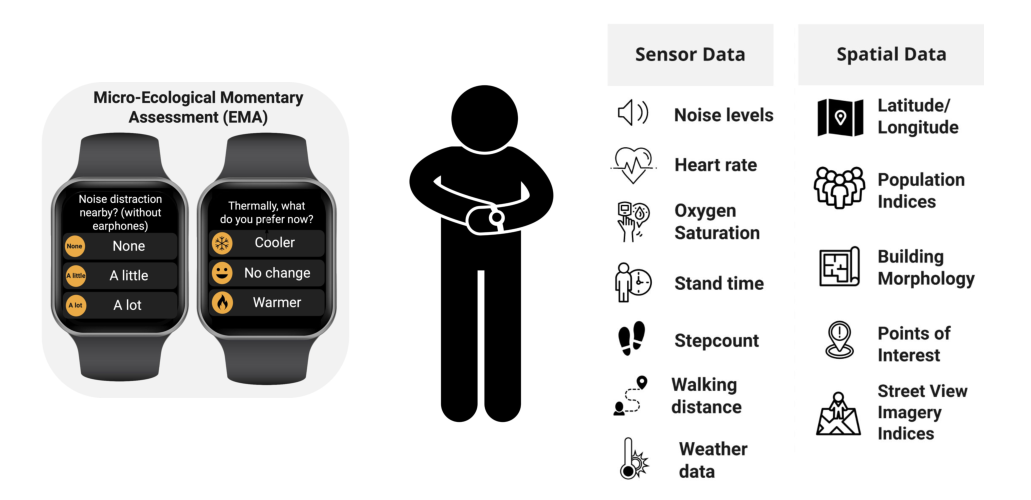
\includegraphics[width=0.92\textwidth]{figures/methods/cozie_study_design.pdf}
% Detailed caption (archived): \caption{Overview of the Cozie Singapore study design, which links crowdsourced smartwatch micro-surveys to contextual data streams. The left side shows the participant-facing smartwatch micro-ecological-momentary-assessment (micro-EMA) interface, where wearers self-report perceptions such as thermal preference (cooler / no change / warmer) and noise directly on the watch. The right side shows the two contextual data streams each response is joined to: wearable sensor data (for example heart rate, step count, and sound level) and urban spatial data tied to the response location.}
\caption{Cozie Singapore study design linking crowdsourced smartwatch micro-surveys (left) to the wearable-sensor and urban spatial data each response is joined to (right).}
\label{fig:cozie-study-design}
\end{figure}

The deployment ran in two phases that differed in how just-in-time intervention messages were triggered.
As summarised in Figure~\ref{fig:cozie-study-design}, each watch-based micro-survey response is time-stamped and geolocated, and is paired with the wearer's onboard physiological signals and with linked outdoor weather and urban-context data.
The present analysis draws on a slightly different prepared dataset from this deployment, comprising 9{,}962 micro-survey responses from 106 participants, and focuses on characterizing the reported experience rather than the intervention outcomes. 

% [PLACEHOLDER: Describe the derived survey-level dataset
% (\texttt{cozie\_sg\_surveys\_with\_health\_aggregates}): 9{,}962 responses,
% 106 participants, 99+ columns. Explain how HealthKit physiological metrics are
% aggregated to a 1-hour pre-survey window and how home locations were recovered.]

% \subsubsection{Micro-survey structure}\label{sec:methods-perception}

% [PLACEHOLDER: List subjective variables --- thermal preference, noise level,
% noise kind, earphones, social context (alone/group), activity --- and their
% response categories.]

Each micro-survey is a short set of questions answered directly on the watch face, shown in Figure~\ref{fig:cozie-microsurvey}.
A response records the participant's thermal preference (\emph{Cooler}, \emph{No change}, or \emph{Warmer}) and the level of nearby noise (\emph{None}, \emph{A little}, or \emph{A lot}).
When noise is present, follow-up questions capture the kind of noise and whether earphones are being worn.
The survey also records the reported location or space type, whether the participant is \emph{Alone} or in a \emph{Group}, and the activity being performed, with the activity options depending on whether the participant is alone or with others.
Several of these questions are conditional, so later items such as noise kind and activity are answered only for the responses that reach them.
% This is what produces the branching flow drawn in Figure~\ref{fig:cozie-microsurvey}.

\begin{figure}[htbp]
\centering
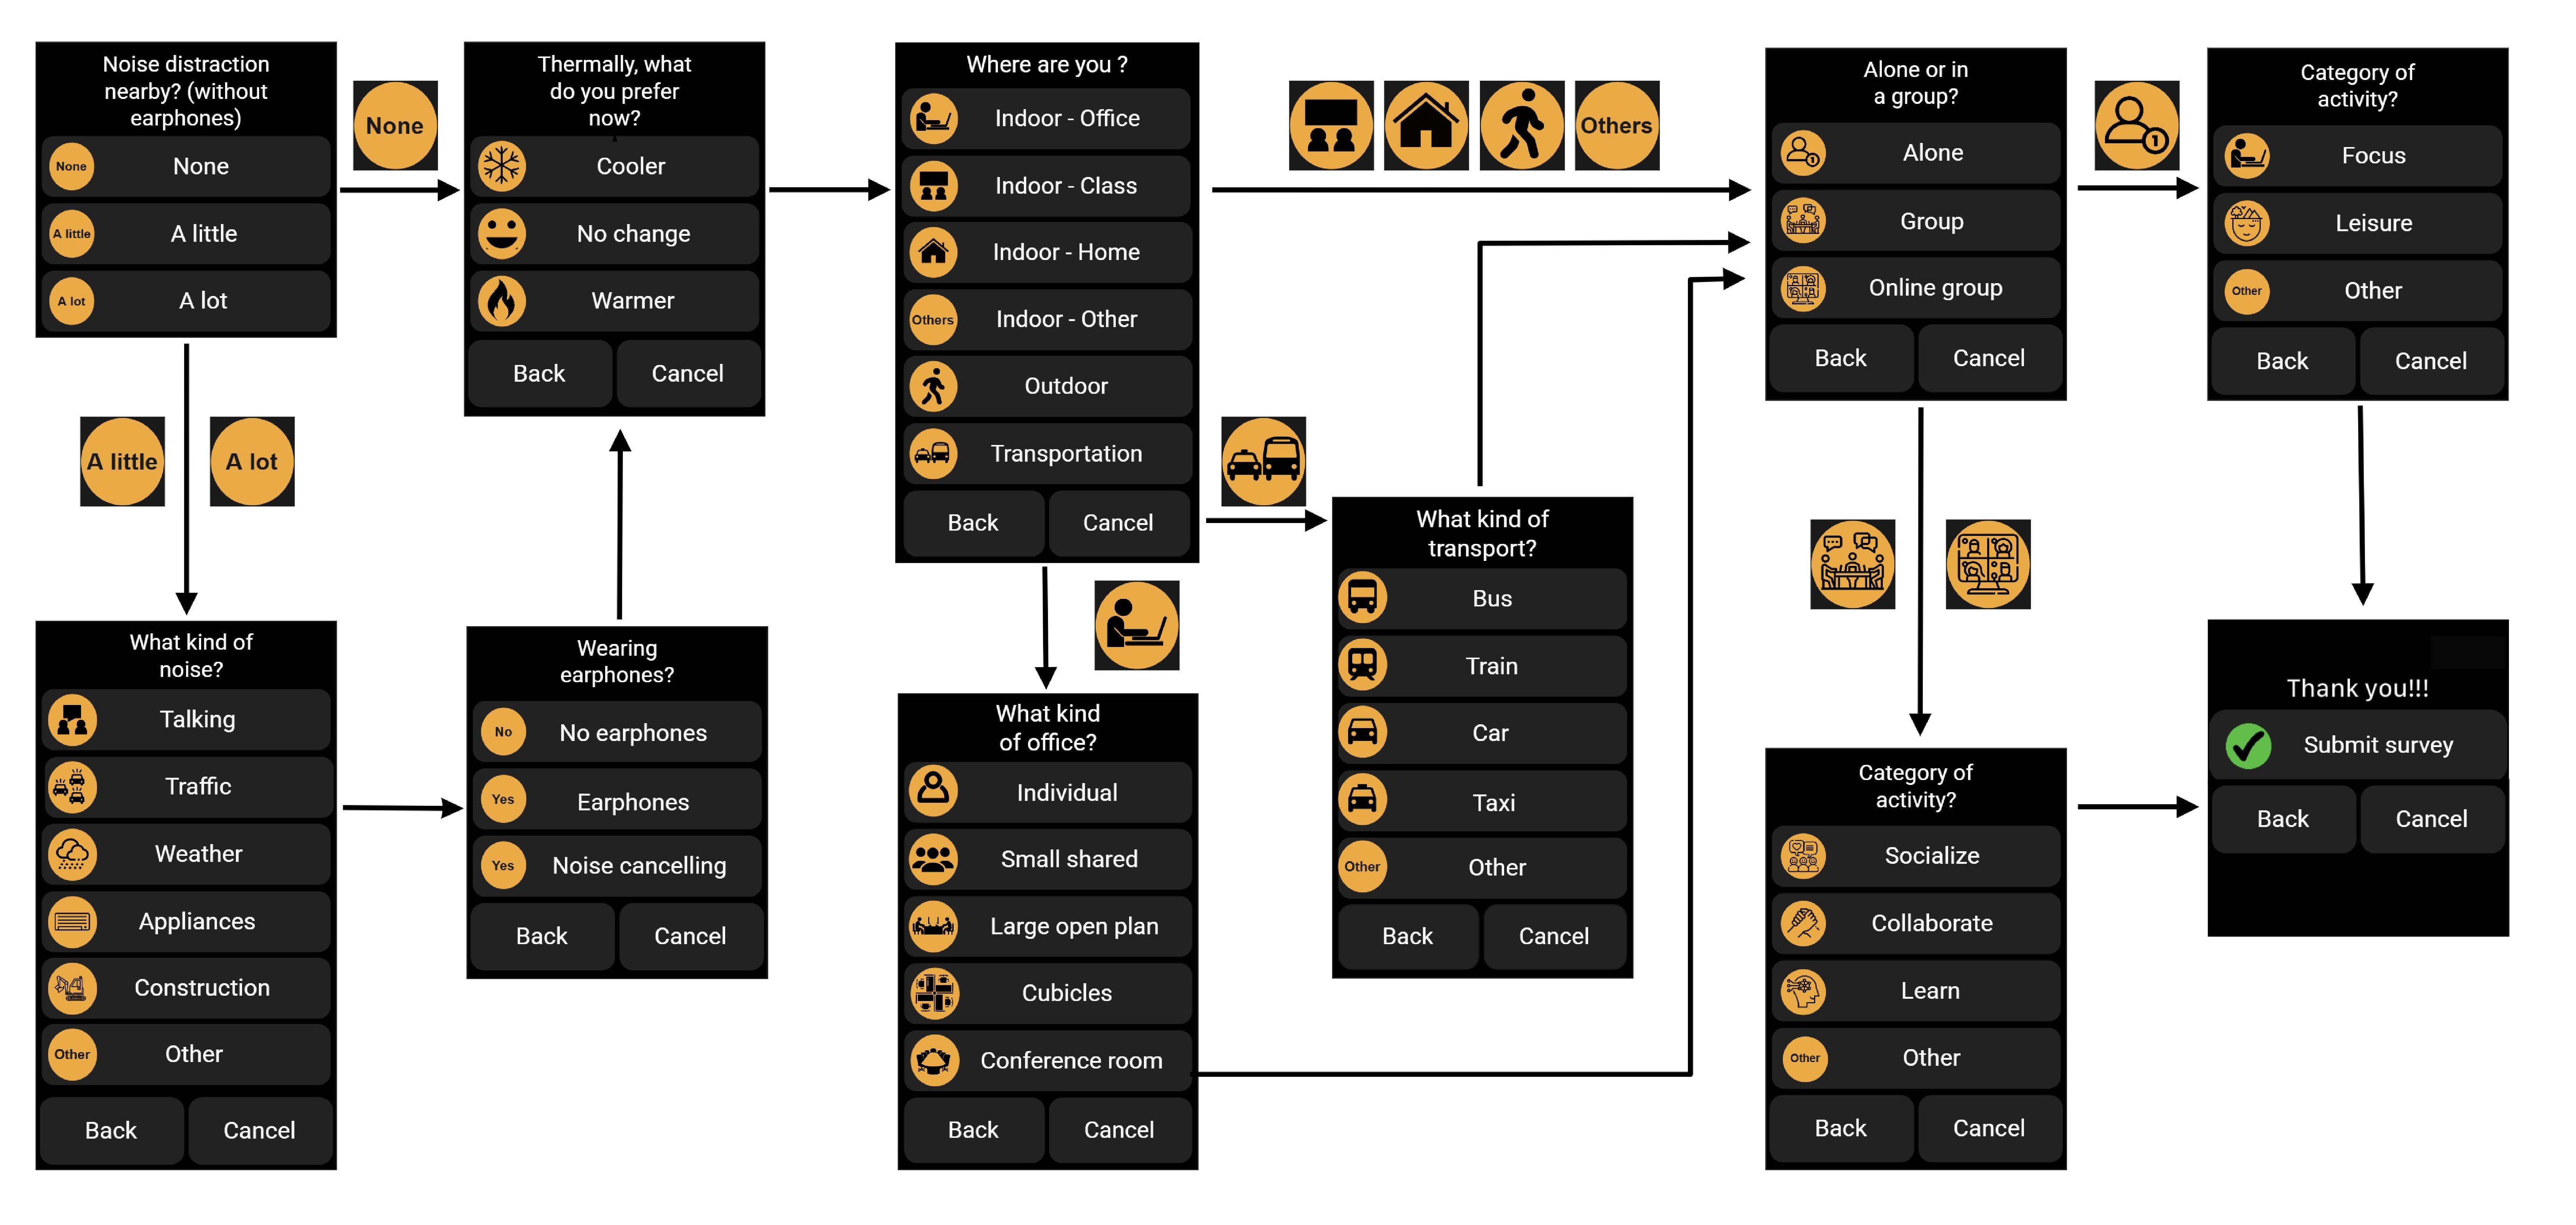
\includegraphics[width=1\textwidth]{figures/methods/cozie_microsurvey.pdf}
% Detailed caption (archived): \caption{The Cozie smartwatch micro-survey interface and its conditional response flow, shown as the sequence of watch screens a participant moves through. Starting from the watch face on the left, a tap opens the survey and advances through the core prompts---perceived noise, thermal preference, location or space type, and social context---with conditional follow-up screens (for example noise type and earphone use when noise is reported, or activity when alone versus in a group) branching from the relevant answers, and ending at a confirmation screen on the right once the response is submitted.}
\caption{Smartwatch micro-survey interface showing the left-to-right flow of watch screens from the core questions and their conditional follow-ups to submission.}
\label{fig:cozie-microsurvey}
\end{figure}

Each geolocated response was linked to a set of urban-context indicators derived with Urbanity, an open-source tool that builds feature-rich urban networks from open geospatial data \citep{Yap2023-xs}.
These indicators summarise the built environment around each response location, including streetscape view indices for greenery, sky, buildings, and roads, together with visual complexity, building count, population, and nearby points of interest across categories such as commercial, food, and recreational uses.
They provide the objective urban characterization used to test whether physical context adds information beyond the self-reported experience.

% \subsubsection{Weather data}\label{sec:methods-weather}
% [PLACEHOLDER: Describe the nearest-station weather aggregation --- air
% temperature, relative humidity, heat index, wind speed, rain, is-raining flag ---
% units and coverage (92--96\%). Note this is ambient, not skin-level, exposure.]

\subsection{Data processing and characterization}\label{sec:methods-eda}

% [PLACEHOLDER: Describe screening and merger of the data from the raw data set found in notebook 00]

The raw deployment data combines high-frequency watch and health streams with the sparser watch-survey responses in a single time-indexed record.
Survey responses were first screened to those triggered on the watch that carried valid, non-zero coordinates falling inside the Singapore bounding box, which produced the 9{,}962-response analysis set.
For each retained response, the seven temporal watch-health streams were aggregated over three pre-survey windows of six hours, one hour, and ten minutes, summarising each window by its count, mean, spread, and extremes, and by an accumulated total for step count, walking distance, and stand time.
The nearest weather-station observations were aggregated over the same three windows, and a heat index was derived from air temperature and relative humidity.
These health and weather aggregates were then merged back onto the survey rows and checked for consistency, yielding one analysis-ready record per response that carries the original survey and location fields alongside the linked physiological, weather, and urban-context features used throughout the analysis.

% [PLACEHOLDER: Describe the EDA strategy from notebook 01 --- univariate survey /
% health distributions, thermal relationships, temporal profiling in Singapore
% local time, and geospatial mapping.]

% The analysis-ready dataset was first characterized descriptively to establish the volume, coverage, and structure of the responses.
% Univariate distributions were computed for each survey item to summarise the balance of reported thermal preference, noise, earphone use, social context, and activity, and the conditional structure of the questionnaire was traced through the set of questions and its branching follow-ups.
% The linked physiological and weather aggregates were profiled across the three pre-survey windows to show their distributions and coverage, and simple bivariate relationships between thermal responses and the linked features were inspected.
% These descriptive views correspond to the survey-response, response-flow, and window-coverage figures presented in the following section (Figures~\ref{fig:data-a1-survey-battery}--\ref{fig:data-a3-weather-windows}).

% [PLACEHOLDER: Describe the characterization methods from notebook 01 ---
% perception fingerprints (row-normalized conditional proportions and lift),
% association and effect size (Kruskal--Wallis $\varepsilon^2$, chi-square /
% Cram\'er's V, Spearman $\rho$)]

% The dataset was then profiled along its temporal, participant, and spatial dimensions to reveal how the responses are distributed in time and space.
% Response timestamps were converted to Singapore local time and profiled by hour of day and day of week, both overall and separately for each reported space type, to expose the weekly cadence and the space-specific timing of submissions.
% Engagement was quantified per participant through response counts and active spans to show how the sample is composed across individuals.
% Finally, the geolocated responses were mapped across Singapore to summarise their spatial density and coverage, corresponding to the geospatial, temporal, and engagement figures in the following section (Figures~\ref{fig:data-b4-response-density-grid-counts}--\ref{fig:data-e2-engagement}).

The reported experience was then characterized against the reported space type using the analysis-ready record described above.
Each response was assigned to one of the space types, and each categorical perception variable was cross-tabulated with the space type to form the contingency tables used below.
Conditional questions such as noise kind and earphone use have lower coverage, so their profiles describe only the responses for which the follow-up was observed.
Because responses are clustered within participants, the significance markers reported below are treated as descriptive screens, and effect sizes and the coherence of contrasts across related variables are used as the primary read-outs. The three methods below produce the perceptual characterization used for analysis.
% shown in Figures~\ref{fig:space-perception-fingerprint}--\ref{fig:space-perception-residuals}.

\subsubsection{Conditional perception fingerprints}\label{sec:methods-fingerprint}
For each space type $s$ and response category $r$, the conditional proportion is the maximum-likelihood estimate of the categorical distribution within that space,
\begin{equation}
\hat{P}(\mathrm{response}=r \mid \mathrm{space}=s) = \frac{n_{rs}}{n_{s}},
\end{equation}
where $n_{rs}$ is the number of responses of category $r$ in space $s$ and $n_{s}$ is the total number of responses in that space.
Each row therefore describes a single space's own response profile and sums to one within each survey variable, which is the fingerprint shown in Figure~\ref{fig:space-perception-fingerprint}.
No smoothing or shrinkage is applied, so cells based on few responses are noisier than their shading suggests.

\subsubsection{Relative distinctiveness through lift}\label{sec:methods-lift}
To separate what is distinctive to a space from what is simply common everywhere, each conditional proportion is divided by the corresponding corpus-wide proportion to give the lift,
\begin{equation}
\mathrm{lift}(r,s) = \frac{P(\mathrm{response}=r \mid \mathrm{space}=s)}{P(\mathrm{response}=r)}.
\end{equation}
A value of one indicates a response that is as common in the space as in the corpus overall, values above one indicate over-representation, and values below one indicate under-representation, as shown in Figure~\ref{fig:space-perception-lift}.

\subsubsection{Association strength and cell-level contrasts}\label{sec:methods-association}
The overall association between space type and each perception was tested with a Pearson chi-square statistic on the $r \times k$ contingency table,
\begin{equation}
\chi^{2} = \sum_{i,j} \frac{(O_{ij}-E_{ij})^{2}}{E_{ij}},
\end{equation}
where $O_{ij}$ and $E_{ij}$ are the observed and expected counts under independence.
Because $\chi^{2}$ grows with sample size, it was rescaled to a bounded effect size using Cram\'er's V,
\begin{equation}
V = \sqrt{\frac{\chi^{2}}{n\,(\min(r,k)-1)}},
\end{equation}
interpreted with conventional descriptive bands (negligible $<0.1$, weak $0.1$--$0.2$, moderate $0.2$--$0.3$, strong $>0.3$).
To identify which individual space and response combinations drive the association, adjusted standardized residuals were computed for each cell,
\begin{equation}
z_{ij} = \frac{O_{ij}-E_{ij}}{\sqrt{E_{ij}\,(1-r_{i}/n)\,(1-c_{j}/n)}},
\end{equation}
where $r_{i}$ and $c_{j}$ are the row and column totals and $n$ is the grand total.
Under independence each $z_{ij}$ is asymptotically standard normal, so cells with $|z|>1.96$, $2.58$, and $3.29$ exceed the conventional $0.05$, $0.01$, and $0.001$ thresholds and mark the space and response pairs shown as over- or under-represented in Figure~\ref{fig:space-perception-residuals}.


% ============================================================================
\section{Results}\label{sec:results}
% ============================================================================

The collected data support the analysis of the volume, coverage, and timing of the responses, to the distributions of the survey and its linked physiological and weather measurements, and then to how the reported experience differs across the everyday spaces in which it was recorded.

\subsection{Data collection, coverage, and temporal characteristics}\label{sec:res-data-collection}

Figure~\ref{fig:data-b4-response-density-grid-counts} shows the mapping of the responses across Singapore.
The densest grid cells sit over residential estates and the NUS university campus, consistent with the roughly 45\% of responses reported from home, while coverage thins quickly toward the periphery even as individual responses still reach the central business district and points along the transport network.
The coverage is therefore broad but uneven, anchored to where participants live and work. 

\begin{figure}[htbp]
\centering
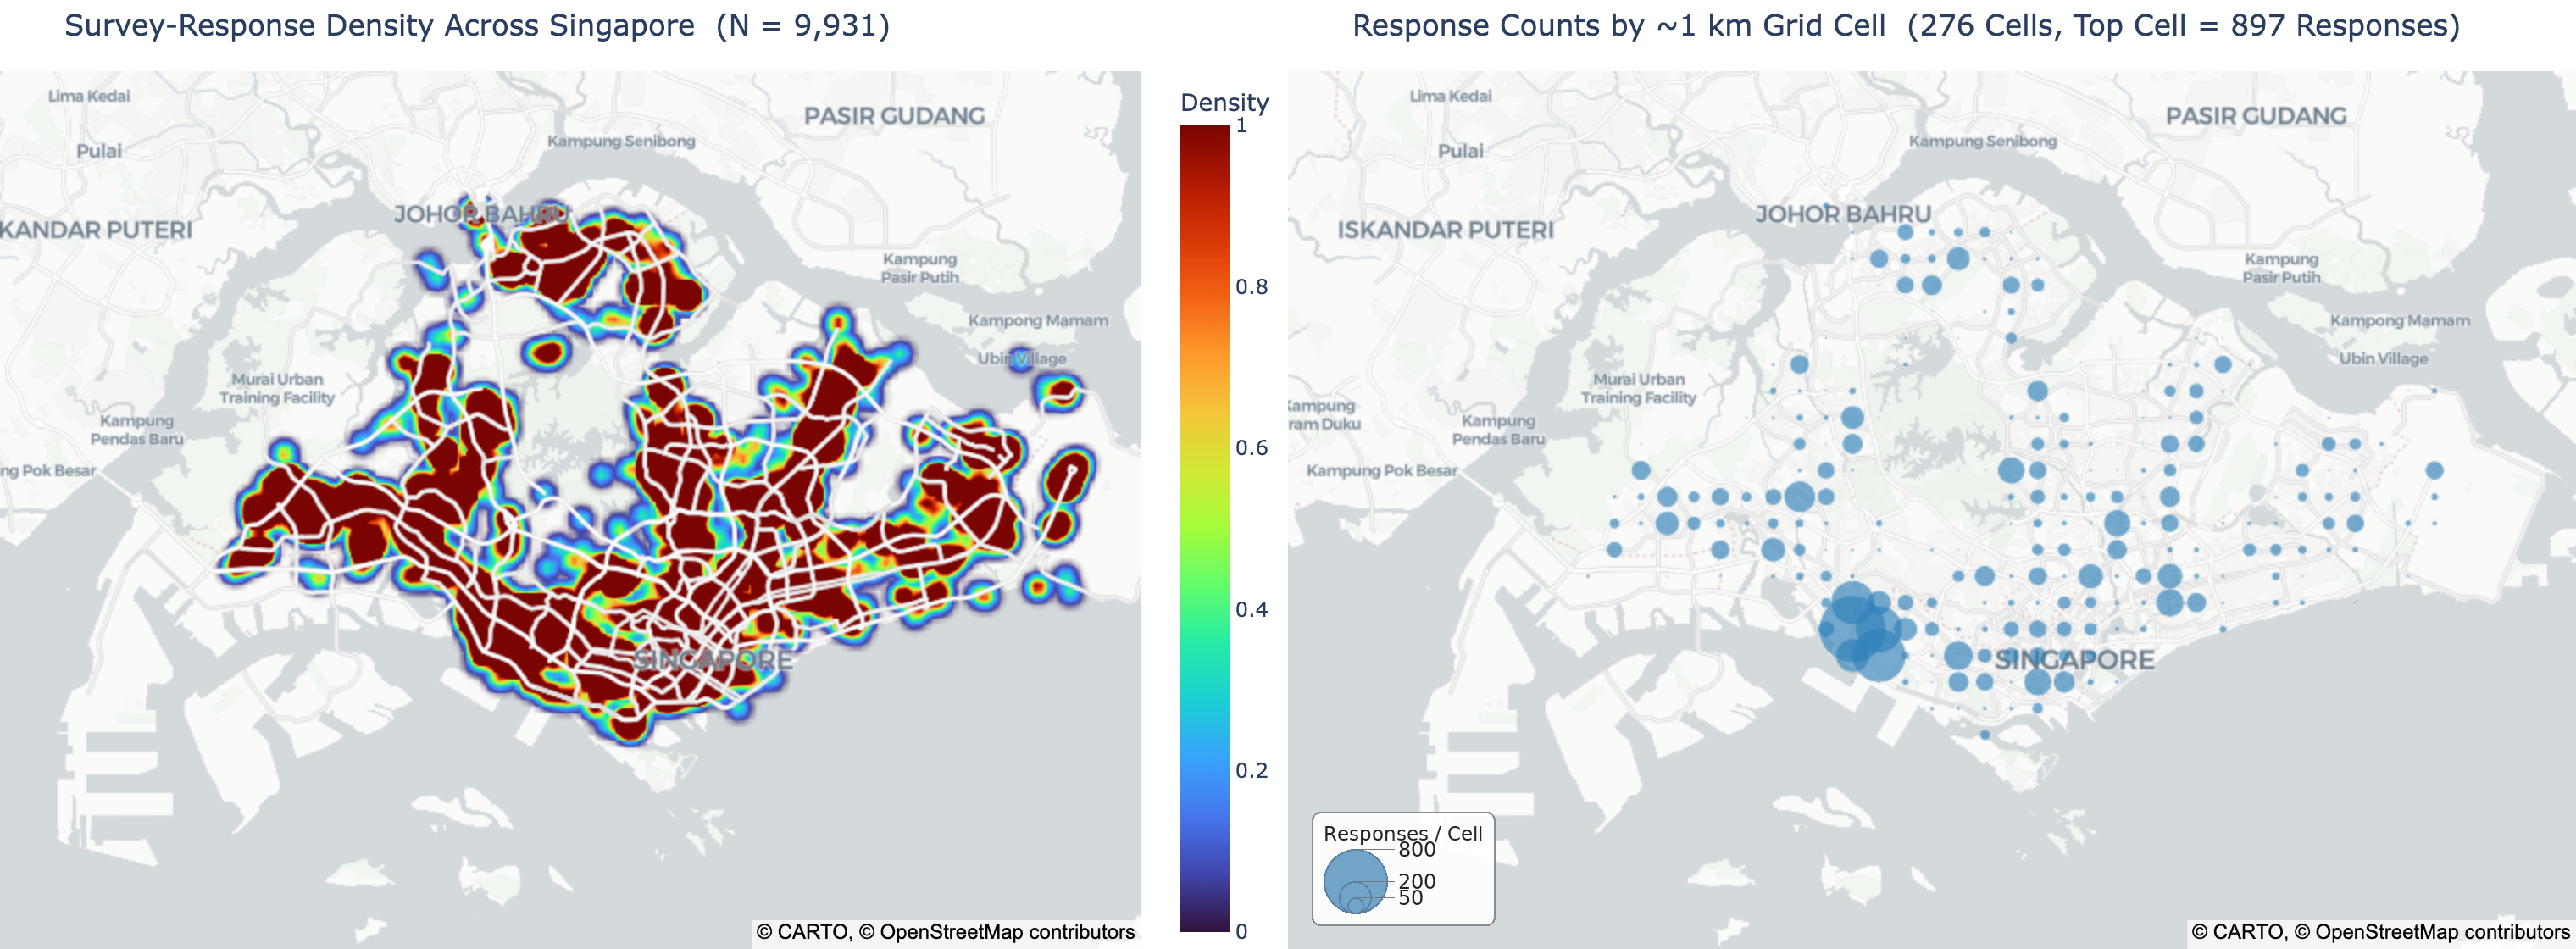
\includegraphics[width=\textwidth]{figures/data_characterization/response_density_and_grid_counts.png}
% Detailed caption (archived): \caption{Spatial coverage of survey responses across Singapore. Left: a kernel-density surface of response locations ($N = 9{,}931$), where warmer shading marks higher response density. Right: the same responses aggregated into approximately 1-km grid cells (276 cells) and drawn as proportional circles, where larger circles denote more responses per cell (top cell 897). Both panels show responses concentrated in the south-west, with lighter coverage across the central, eastern, and northern parts of the island.}
\caption{Spatial coverage of survey responses across Singapore, shown as a kernel-density surface of response locations ($N = 9{,}931$; left) and response counts aggregated into approximately 1-km grid cells (276 cells, top cell 897 responses; right).}
\label{fig:data-b4-response-density-grid-counts}
\end{figure}

Figure~\ref{fig:data-e2-engagement} illustrates the breakdown of data collection across the cohort of 106 participants.
Contribution is spread evenly enough that no small group dominates the dataset, with a median of 98 responses per person, close to the 100-survey target, and the most active tenth of participants supplying only about 12\% of the total.
The range from 17 to 158 responses does mean that some participants are somewhat unequally represented, the analyses that follow rely on within-space proportions and effect sizes rather than raw response counts.

\begin{figure}[htbp]
\centering
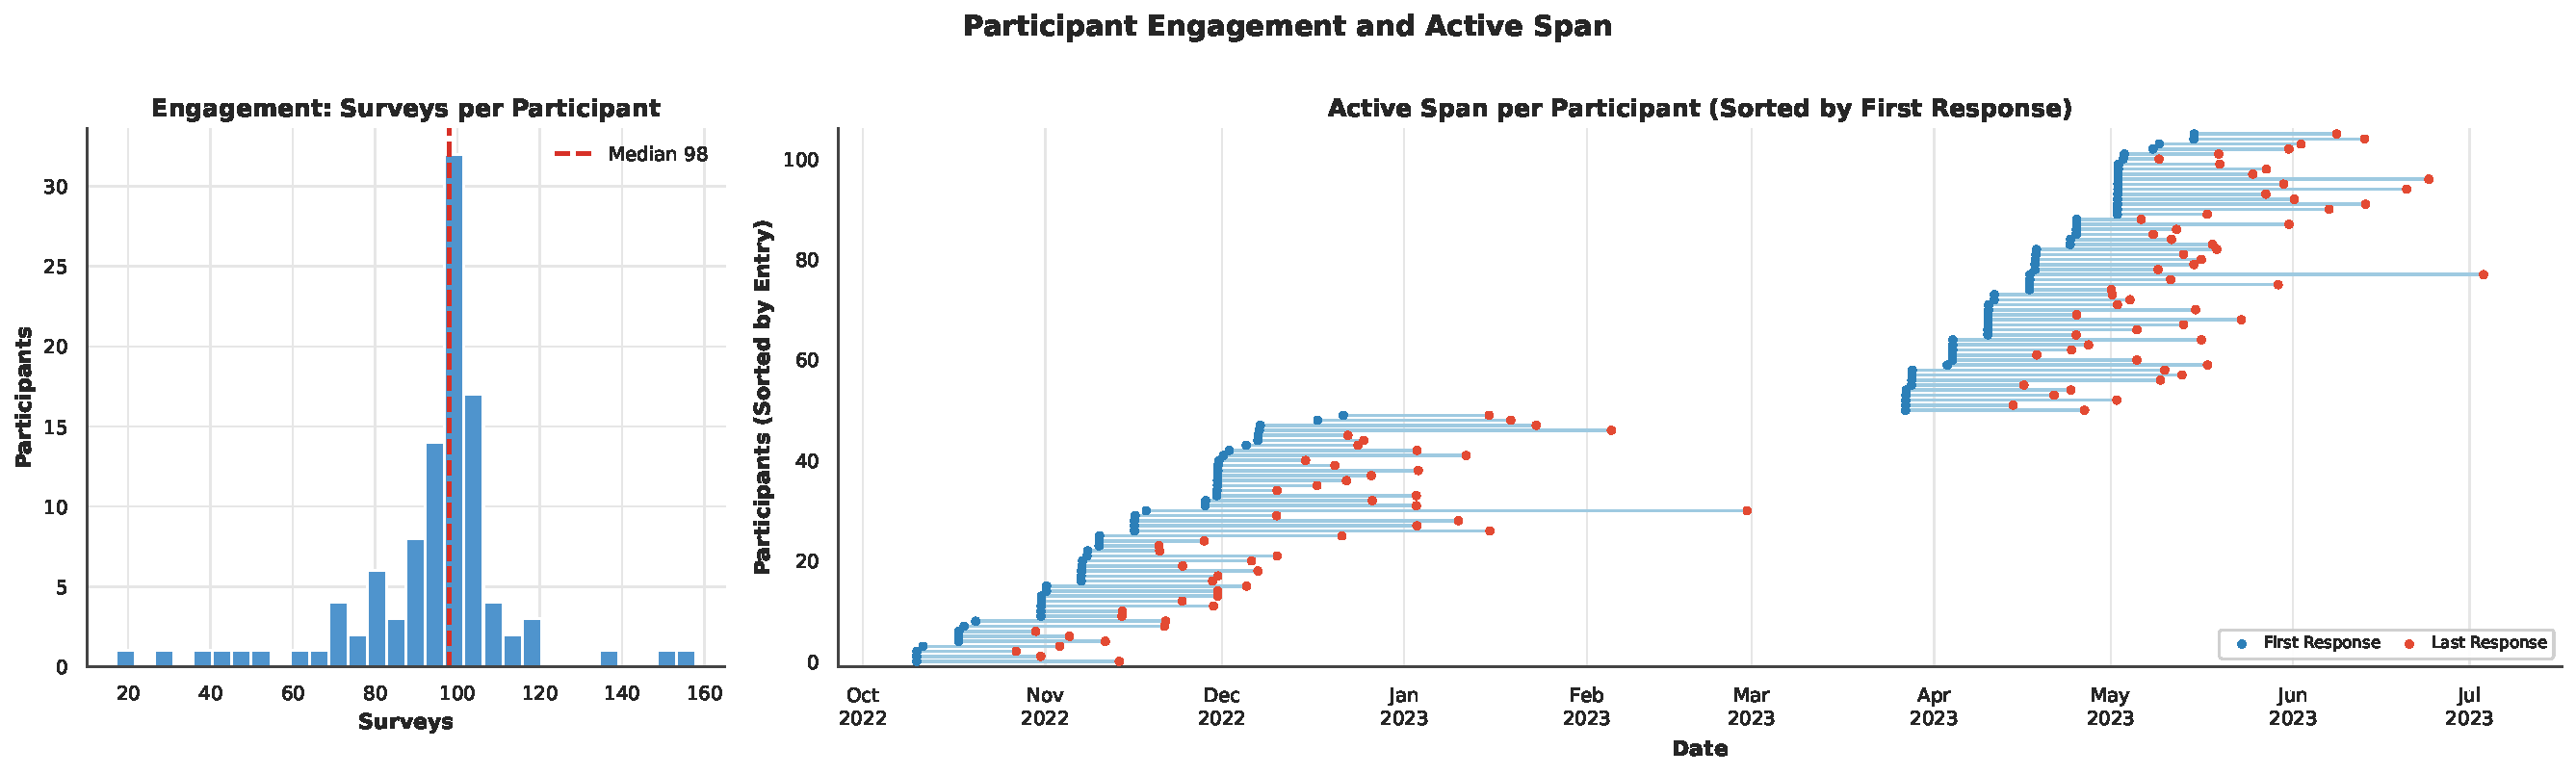
\includegraphics[width=\textwidth]{figures/data_characterization/participant_engagement.pdf}
% Detailed caption (archived): \caption{Participant engagement and active survey span over the deployment. Left: the distribution of completed surveys per participant, with a median of 98 responses. Right: the active span of each of the 106 participants, drawn as one horizontal segment per participant from first to last response and sorted by entry date, across the October 2022--July 2023 collection period.}
\caption{Participant engagement over the deployment: the distribution of surveys per participant (left; median 98) and each participant's active span from first to last response (right).}
\label{fig:data-e2-engagement}
\end{figure}

The temporal cadence in Figure~\ref{fig:data-d2-temporal-cadence} reflects a protocol built around the working day.
Responses concentrate sharply between 9\,AM and 7\,PM and peak in the mid-afternoon, and weekdays account for all but about 17\% of the data, so the dataset captures waking, active hours far more than nights or weekends.
The calendar-week panel shows the response volume rising and falling with the phased recruitment of participants.

\begin{figure}[htbp]
\centering
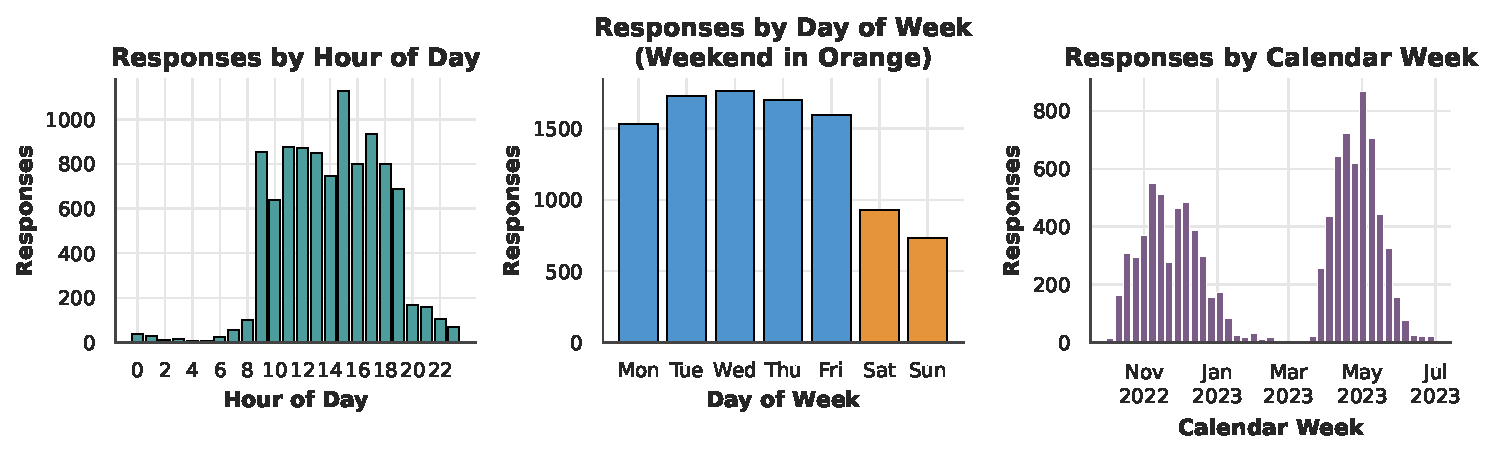
\includegraphics[width=\textwidth]{figures/data_characterization/weekly_temporal_cadence.pdf}
% Detailed caption (archived): \caption{Temporal cadence of survey responses in Singapore local time, shown as three panels. Left: responses by hour of day. Middle: responses by day of week, with weekend days highlighted. Right: responses by calendar week across the deployment. Together the panels show when responses were contributed over the day, the week, and the study period.}
\caption{Temporal cadence of survey responses in Singapore local time by hour of day (left), day of week (middle), and calendar week (right).}
\label{fig:data-d2-temporal-cadence}
\end{figure}

Timing is normalised within each space type in Figure~\ref{fig:data-d4-space-time}, so it reads as a set of temporal signatures for when each kind of space is used.
Offices and classrooms are almost only weekday, daytime settings, with about 96\% of office responses on weekdays, while home stretches into the evening and holds the largest weekend share of any space.
The commute spaces give the sharpest signatures, as outdoor and transportation responses break from the mid-afternoon indoor peak and rise in the early evening around 18:00 to 19:00.
Timing alone already begins to separate the spaces before any perception is considered.

\begin{figure}[htbp]
\centering
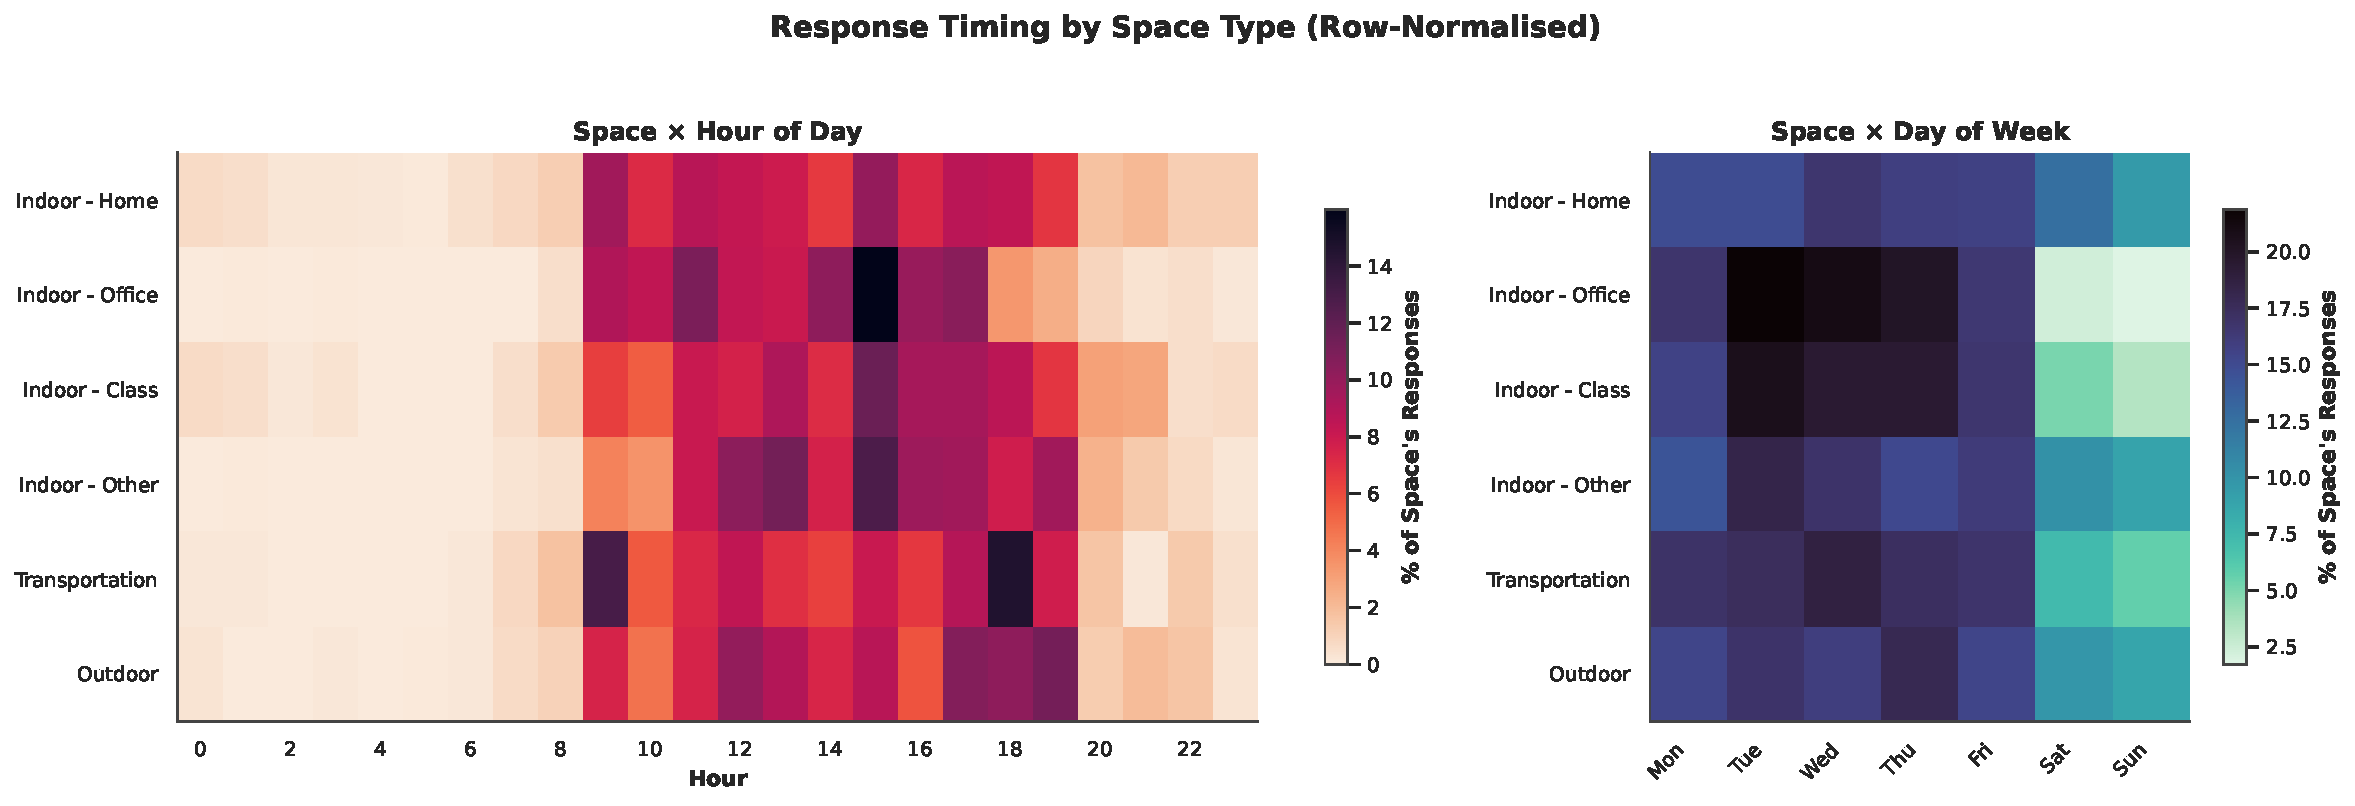
\includegraphics[width=\textwidth]{figures/data_characterization/space_type_timing_heatmaps.pdf}
% Detailed caption (archived): \caption{Response timing by space type, shown as two row-normalised heatmaps in which each row is one of the six reported space types and colour encodes the share of that space's responses. Left: space type by hour of day (columns spanning 0--23\,h). Right: space type by day of week (Monday--Sunday). Row-normalisation lets each space's own temporal profile be read independently of how many responses it contributed.}
\caption{Row-normalised response timing by space type, showing each space's share of responses across hour of day (left) and day of week (right).}
\label{fig:data-d4-space-time}
\end{figure}



\subsection{Survey responses and linked temporal data coverage}\label{sec:res-survey-overview}
Figure~\ref{fig:data-a1-survey-battery} gives the overall distribution of every question, and read together the panels sketch the typical moment a participant reported.
Thermal preference is strongly asymmetric.
A small majority want \emph{No change} (54\%), almost all of the rest want to be \emph{Cooler} (40\%), and \emph{Warmer} is rare (6\%).
This is the expected pattern for a warm, humid climate, though it also reflects that many indoor spaces are air-conditioned rather than exposed to the outdoor weather.
Perceived noise is more balanced, with roughly equal shares reporting \emph{None} (46\%) and \emph{A little} (44\%) and only about one in ten reporting \emph{A lot}.
Noticing some noise is the norm, while strong distraction is uncommon.
Where noise is present, the follow-up question attributes it most often to people talking (44\% of noise-kind responses), well ahead of appliances and traffic, so the main acoustic nuisance in this cohort is human rather than mechanical.

The other panels place these responses in context.
Most responses come from home (45\%), participants are usually \emph{Alone} (72\%) rather than in a \emph{Group}, and the activity questions show focused work and leisure in solitary moments and socialising in group ones.
Earphone use is uncommon even though the question is reached in about half of surveys, as most of those responses report \emph{No earphones} and active noise cancelling is rare.
Participants therefore seem to tolerate rather than mask their sound environment.
The coverage panel shows why the linked analysis is feasible, since the one-hour pre-survey window carries weather for about 96\% of surveys and heart rate, movement, and measured noise for roughly 90\%.
Nearly every self-report has matching sensor data.

\begin{figure}[htbp]
\centering
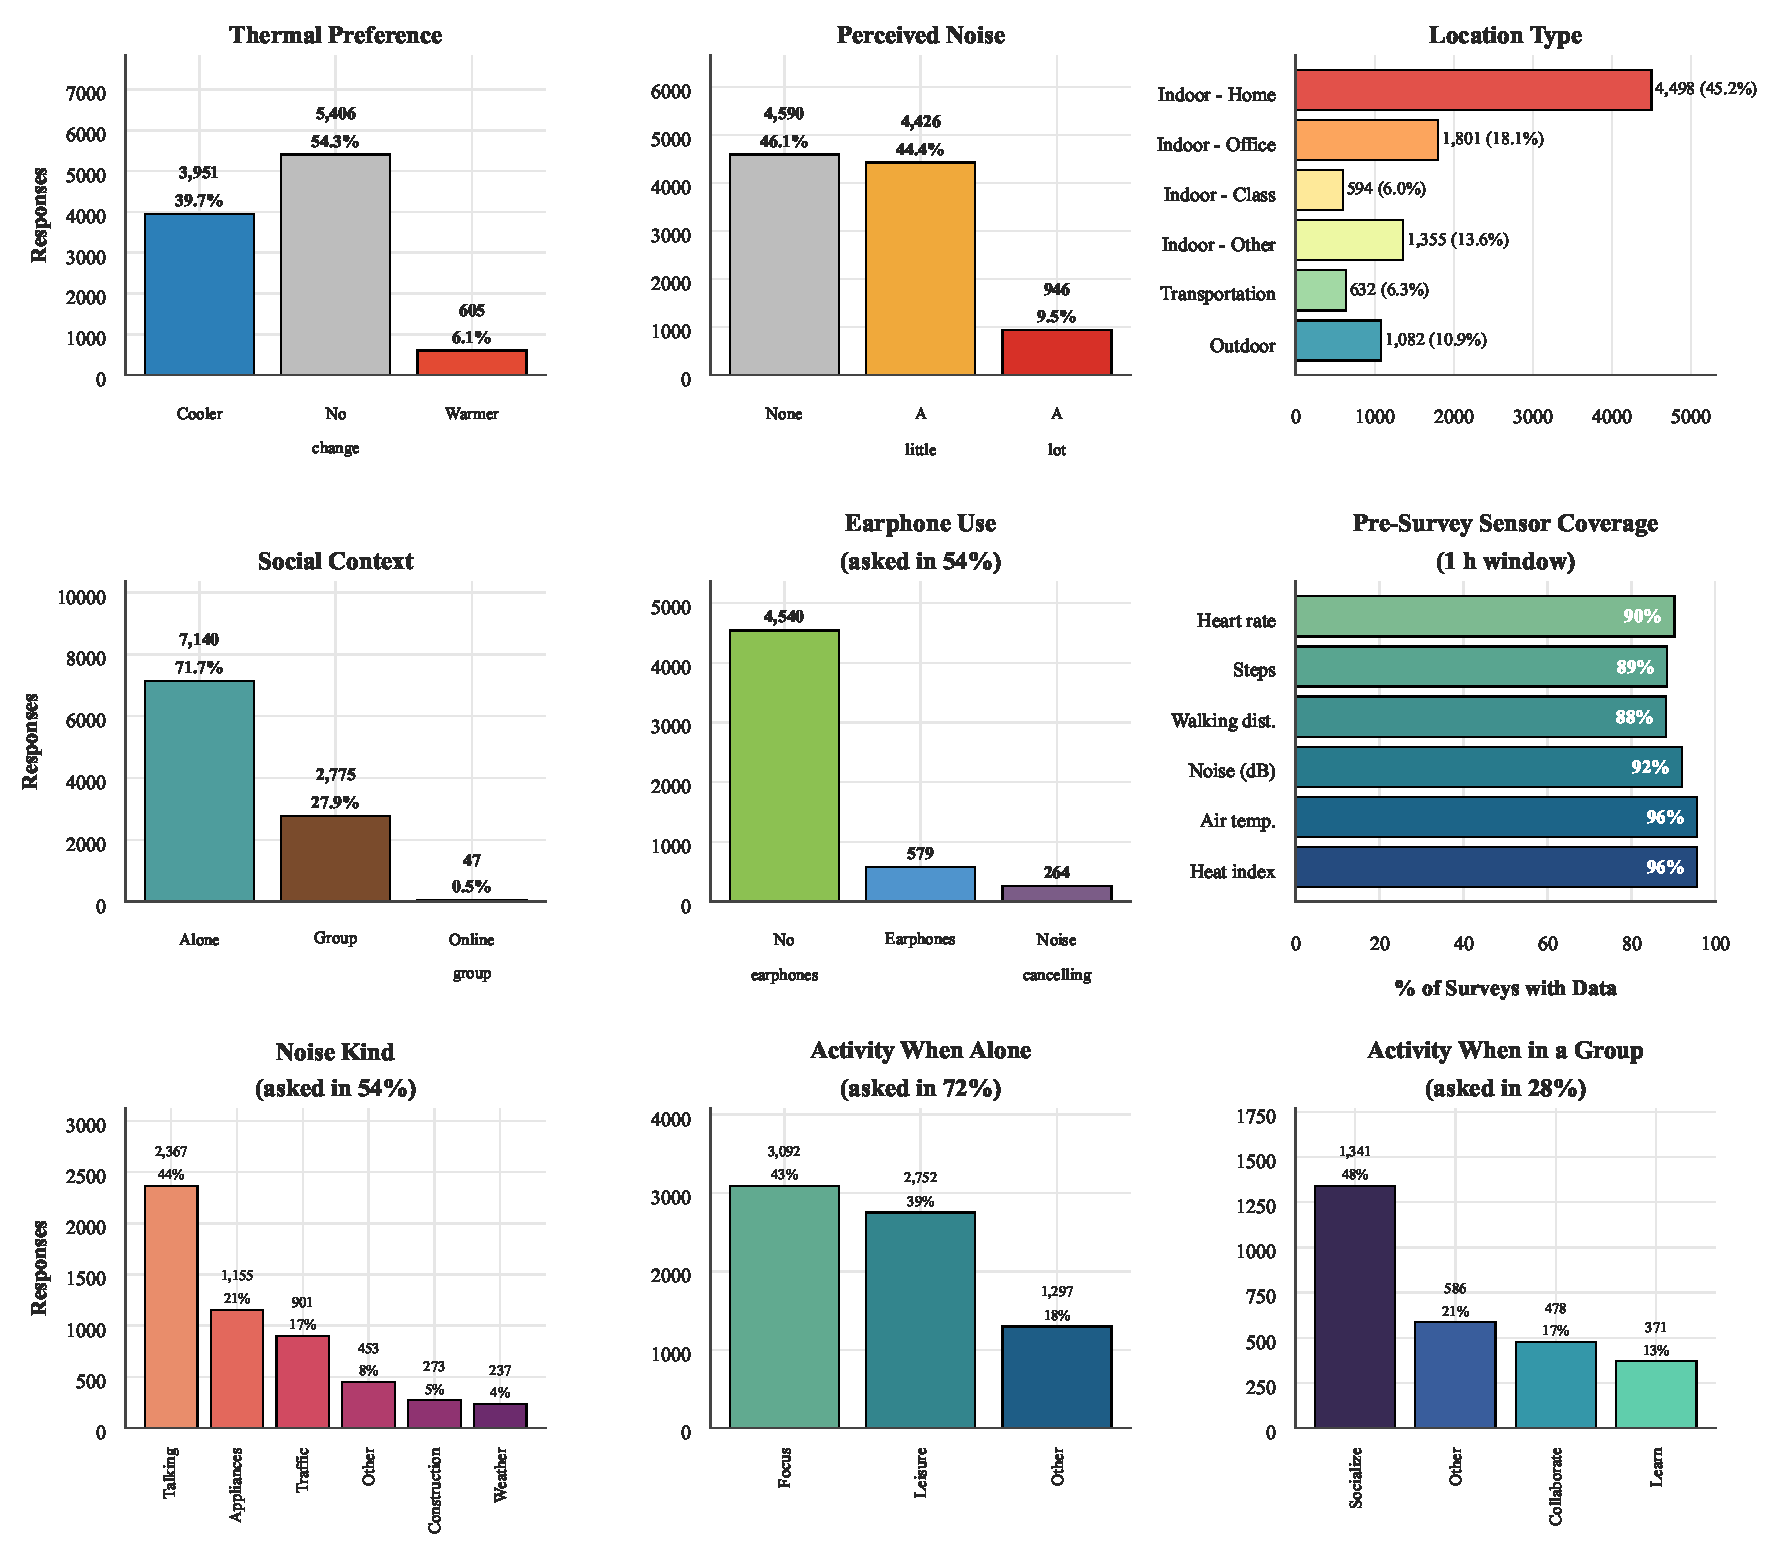
\includegraphics[width=\textwidth]{figures/data_characterization/survey_battery_and_coverage.pdf}
% Detailed caption (archived): \caption{Survey response battery and pre-survey sensor coverage ($N = 9{,}962$ responses, 106 participants), arranged as a $3\times3$ grid of panels. Eight bar-chart panels give the response distribution for one survey item each---thermal preference, perceived noise, location type, and social context (always asked), together with the conditional follow-ups earphone use, noise kind, activity when alone, and activity when in a group (each annotated with the share of surveys in which it was asked). The remaining panel reports pre-survey sensor coverage: the percentage of surveys with linked data in a 1-hour window for heart rate, steps, walking distance, sound level, air temperature, and heat index.}
\caption{Response distributions for each survey item and pre-survey linked-sensor coverage ($N = 9{,}962$ responses, 106 participants).}
\label{fig:data-a1-survey-battery}
\end{figure}

The same responses appear as a flow through the questions in Figure~\ref{fig:survey-response-flow}, which makes the conditional structure clearer than the separate bars can.
Reading from left to right, each answer splits into the next question, the conditional branches such as noise kind and earphones carry only the half of responses that reach them, and activity divides by whether the participant is \emph{Alone} or in a \emph{Group}.
The ribbon widths are drawn to scale, so the proportion of every category can be compared in a single view.
The common home, solitary, and \emph{No change} or \emph{Cooler} responses form the thick central spine, and the rarer categories taper into thin branches.

\begin{figure}[htbp]
\centering
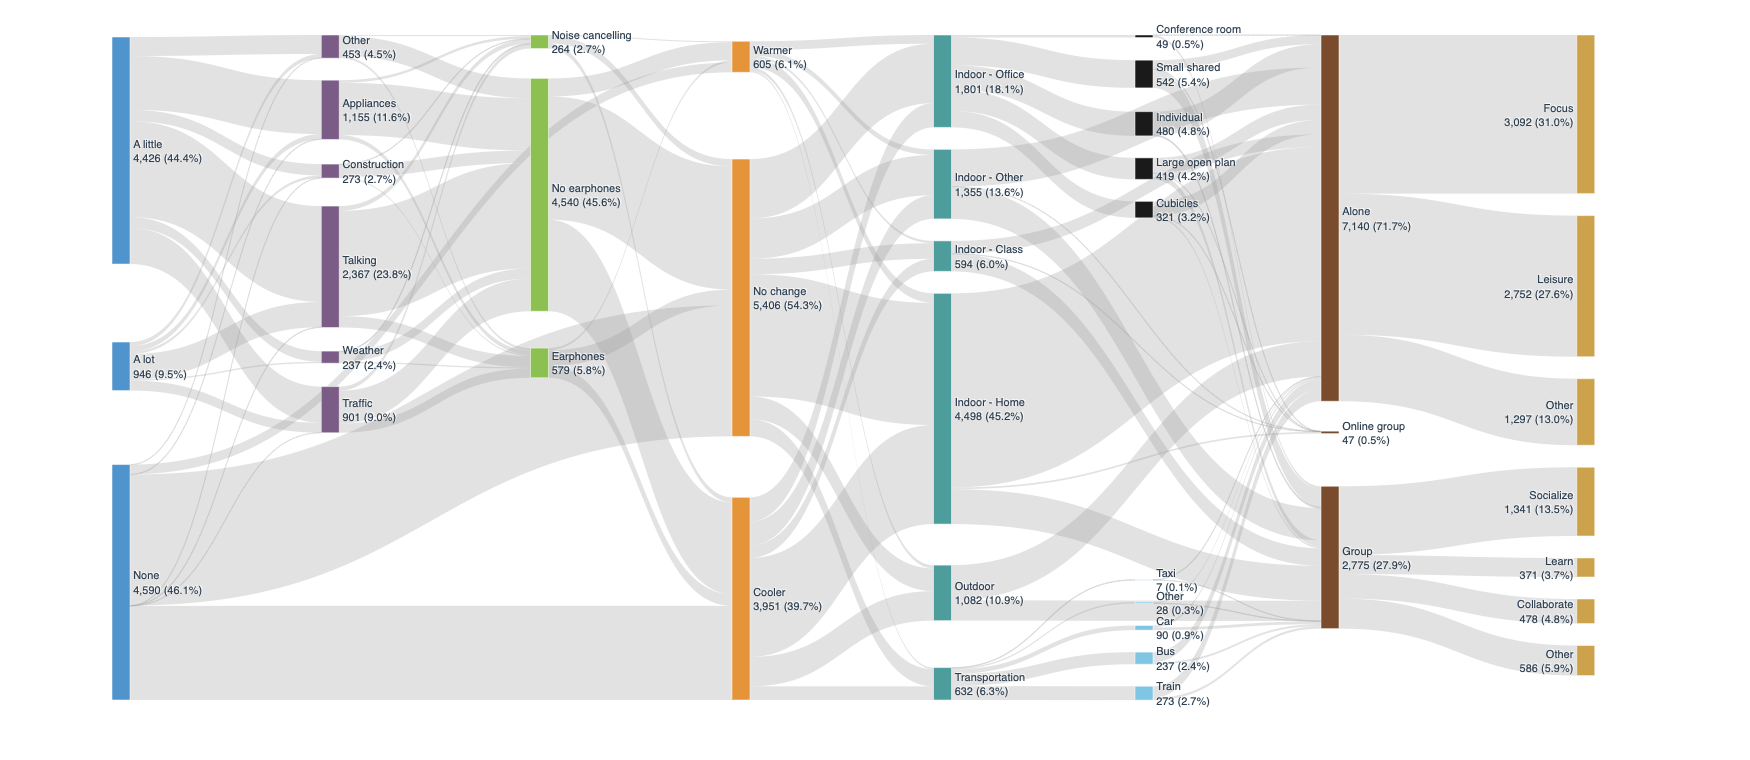
\includegraphics[width=1.1\textwidth]{figures/data_characterization/cozie-sankey-organized.png}
% Detailed caption (archived): \caption{Conditional response flow through the watch-survey questionnaire, drawn as a left-to-right Sankey diagram. Nodes are answer categories and the width of each band is proportional to the number of responses following that path. Reading from left to right, responses fan out from the entry question through perceived noise and its follow-ups, thermal preference, location type, and social context, so that the thickness and branching of the ribbons reveal the most common combinations of answers.}
\caption{Sankey diagram of the conditional response flow through the questionnaire, with band width proportional to the number of responses along each path.}
\label{fig:survey-response-flow}
\end{figure}

The linked wearable-health streams appear in Figure~\ref{fig:data-a2-health-windows}, each summarised over the six-hour, one-hour, and ten-minute windows before a survey.
The window matters most for the movement metrics.
Median step count and walking distance fall as the window narrows, from about 85 to 42 steps per reading between the six-hour and ten-minute windows, because a short look-back captures only the last few minutes of activity.
Heart rate is far more stable at roughly 80\,bpm across all three windows.
Coverage moves the other way and limits how tight the window can be.
The six-hour window carries movement and noise for over 95\% of surveys, but at ten minutes audio coverage falls to about a third and step coverage to little more than half.
Resting heart rate and blood-oxygen streams are sparse in every window.
The one-hour window is used as the working aggregate throughout, since it keeps coverage near 90\% while staying close to the moment of the survey.

Figure~\ref{fig:data-a3-weather-windows} summarizes the nearest-station outdoor weather over the same windows and its distributions are narrow and stable, as expected for an equatorial climate.
Air temperature has a median near 29\,\textdegree C and relative humidity near 73\%, which give a heat index around 34\,\textdegree C that changes little across the windows.
The outdoor thermal environment is consistently warm whatever the look-back length.
Rainfall is the one strongly window-dependent feature because it accumulates over time, with about 28\% of six-hour windows containing some rain against only 5\% of ten-minute windows.
These values describe outdoor conditions at a station a median of roughly 3\,km from the response.
As noted above, they are not the participant's actual microclimate, which is often indoor and air-conditioned.

\begin{figure}[htbp]
\centering
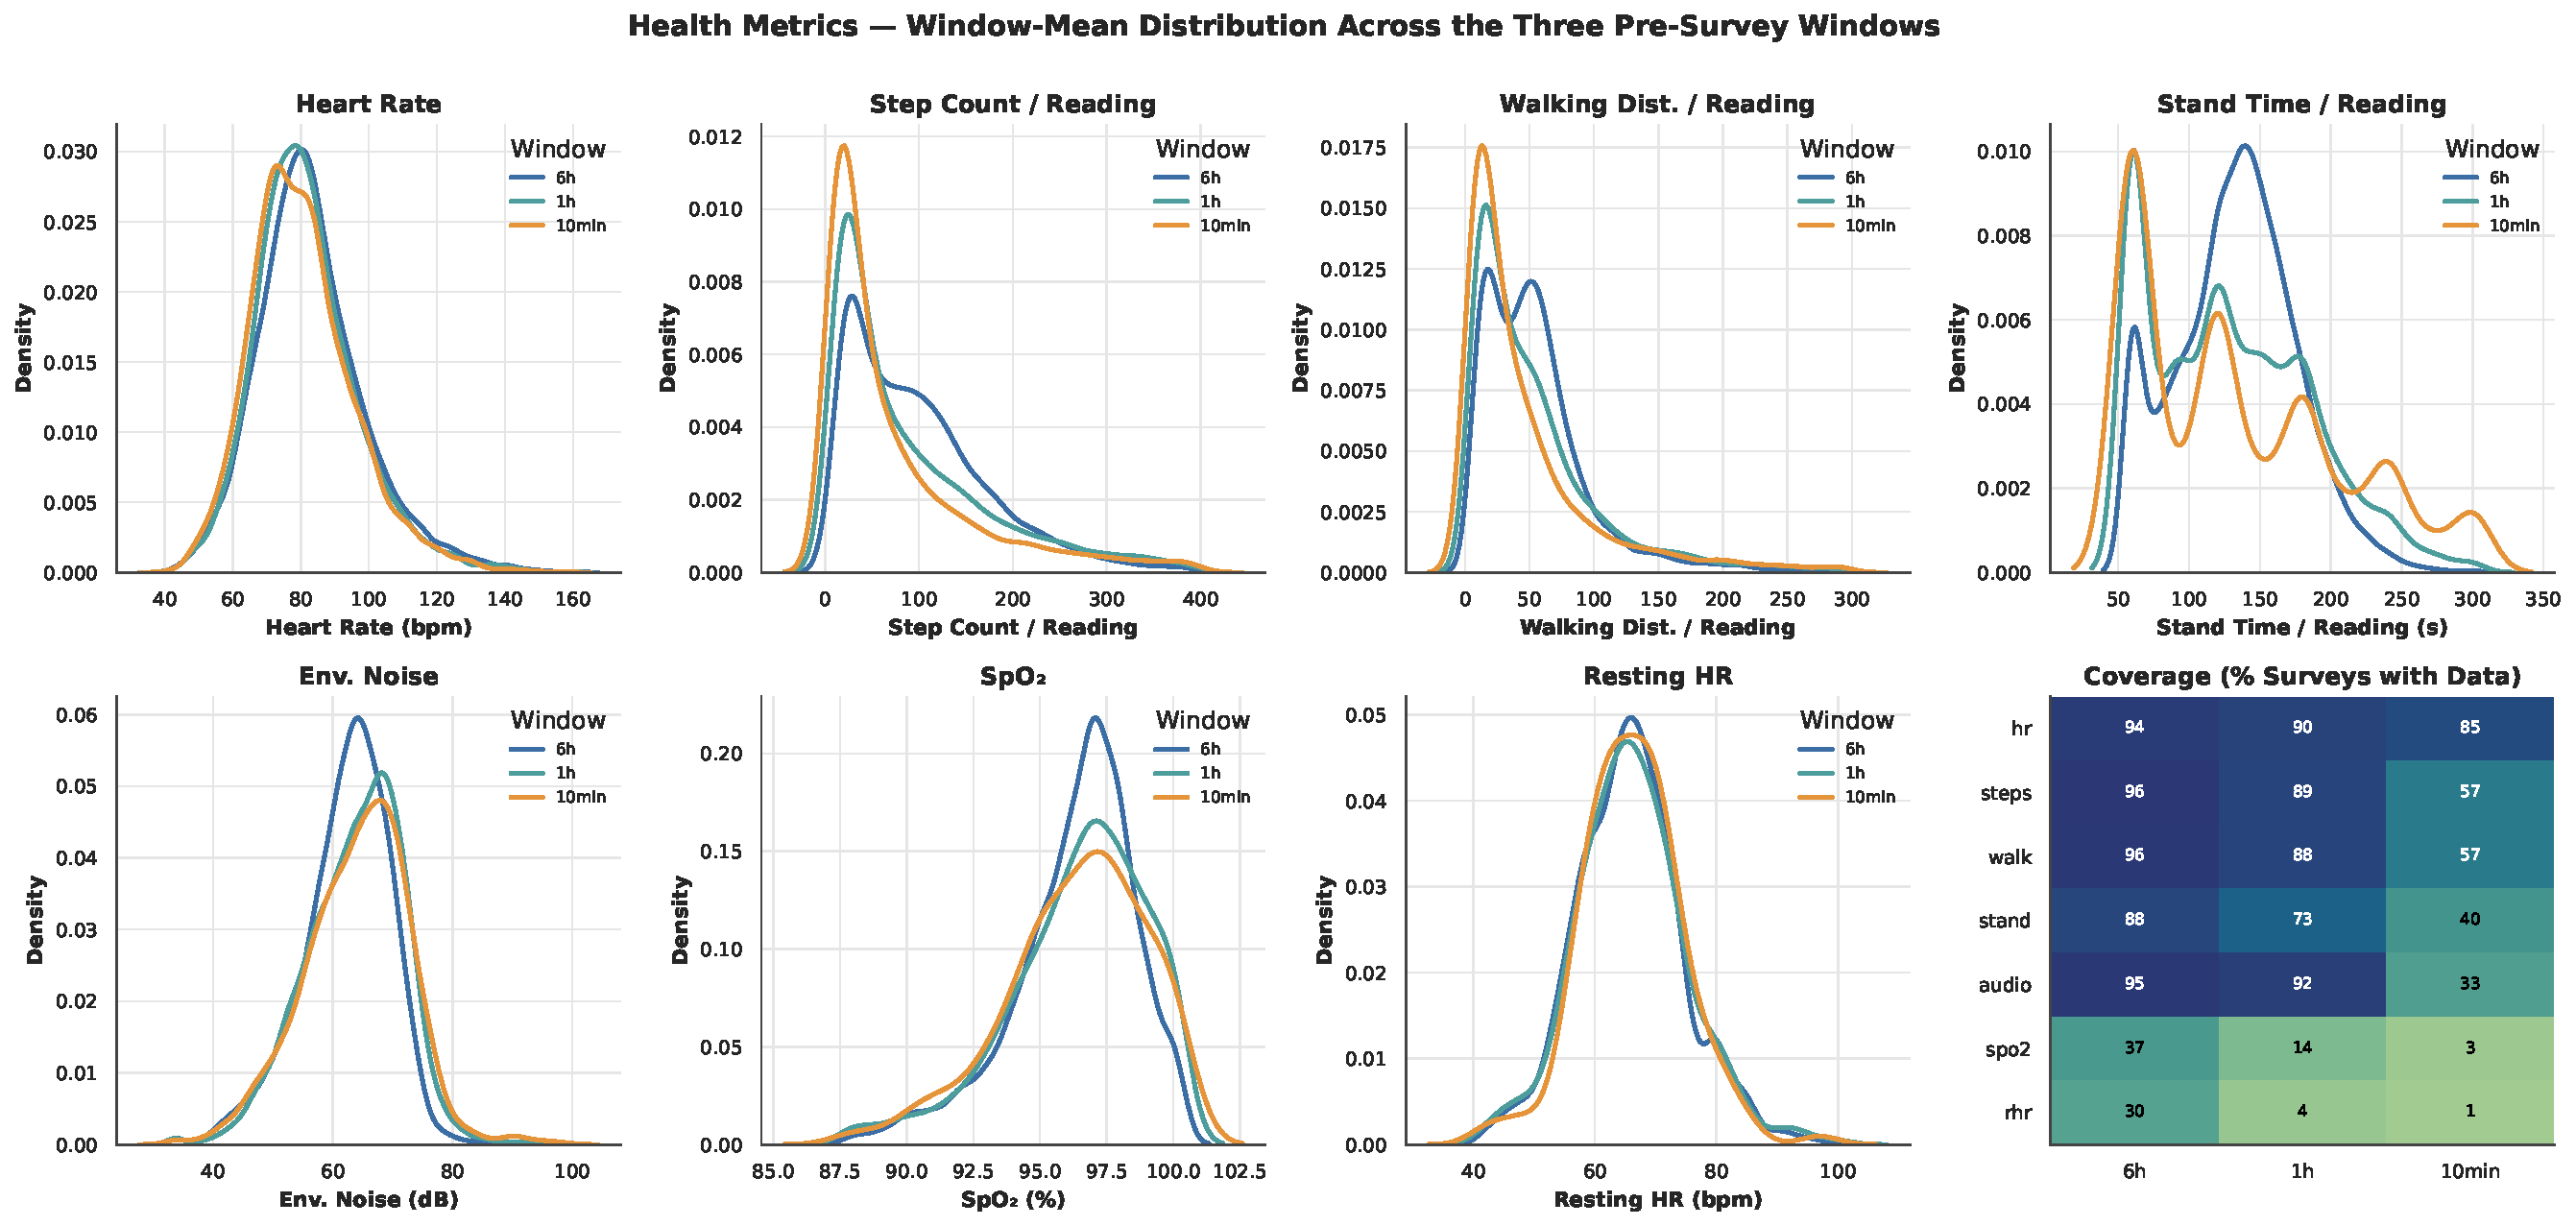
\includegraphics[width=\textwidth]{figures/data_characterization/wearable_health_windows.pdf}
% Detailed caption (archived): \caption{Distributions of wearable-health metrics over three pre-survey aggregation windows. Left: heart rate (bpm). Right: step count per reading. In each panel the three overlaid density curves correspond to the 10-minute, 1-hour, and 6-hour windows preceding each survey, showing how the aggregation window changes the distribution of the linked physiological signal.}
\caption{Distributions of pre-survey wearable-health metrics across the 10-minute, 1-hour, and 6-hour aggregation windows: seven wearable health and audio streams as overlaid per-window density curves, plus a metric-by-window data-coverage heatmap.}
\label{fig:data-a2-health-windows}
\end{figure}

\begin{figure}[htbp]
\centering
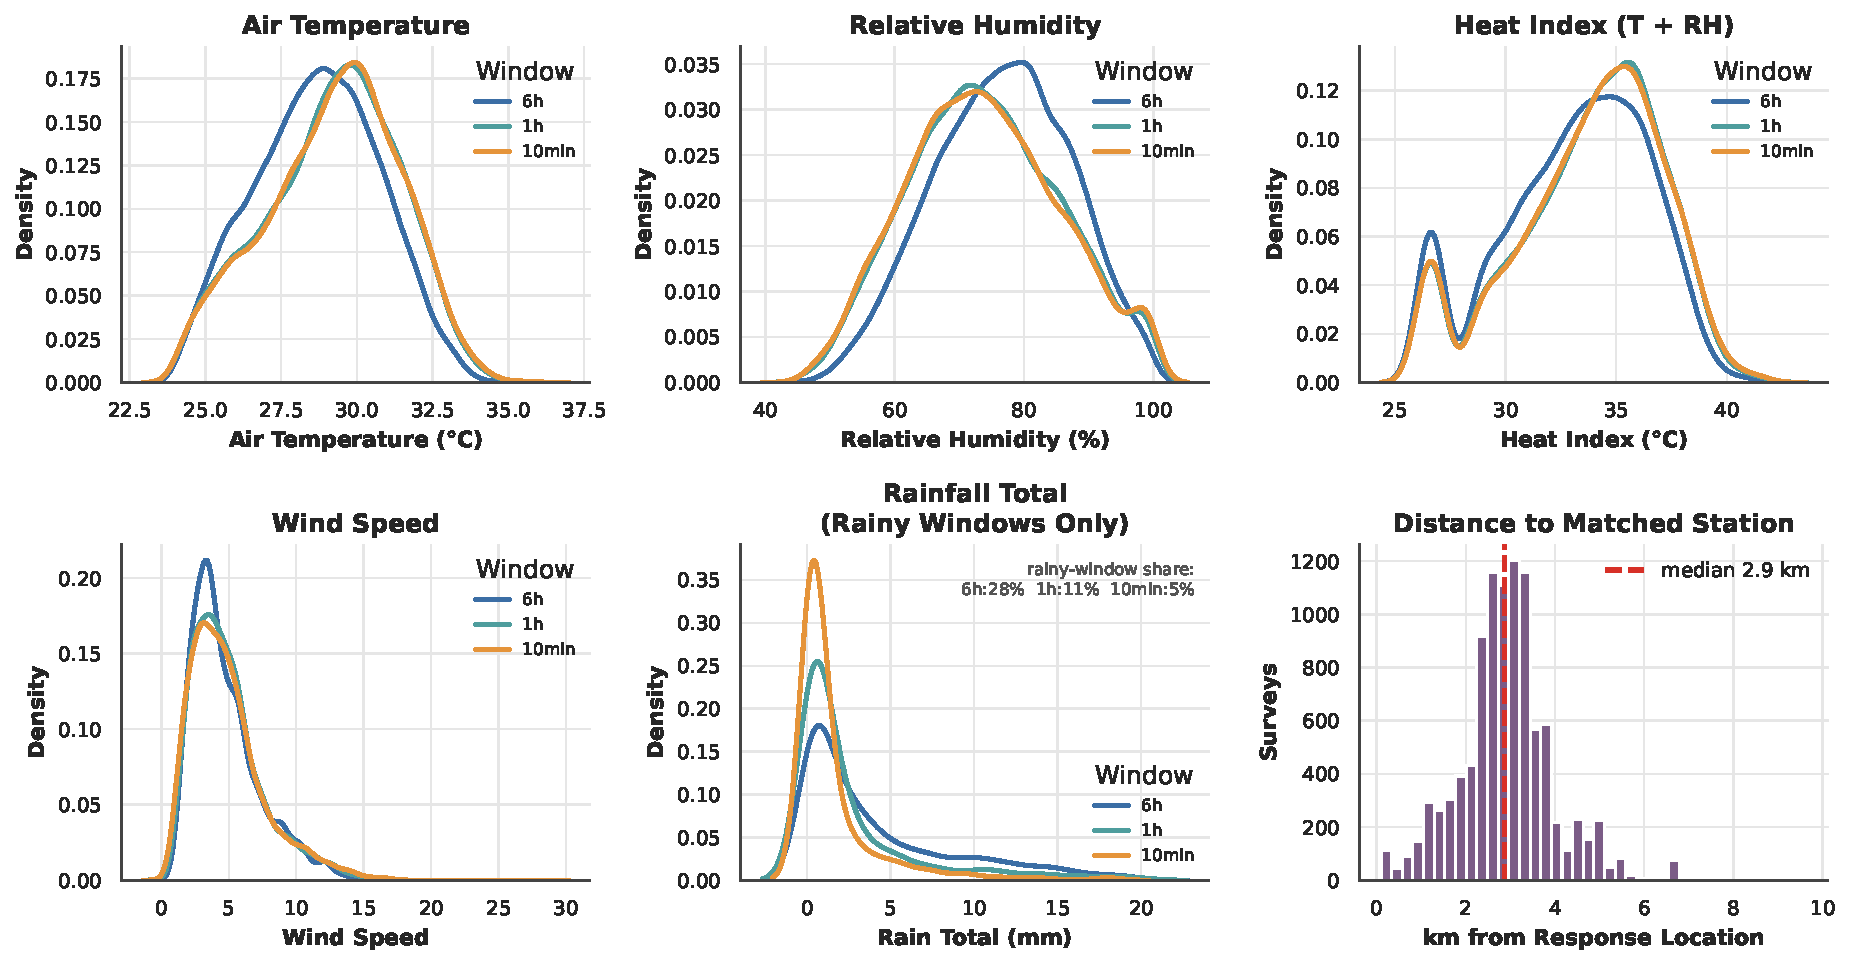
\includegraphics[width=\textwidth]{figures/data_characterization/outdoor_weather_windows.pdf}
% Detailed caption (archived): \caption{Nearest-station outdoor ambient weather across the three pre-survey aggregation windows, arranged as a $2\times3$ grid. Five panels give density distributions for air temperature, relative humidity, heat index (derived from temperature and humidity), wind speed, and rainfall total (over rainy windows only, with the rainy-window share noted), each overlaying the 10-minute, 1-hour, and 6-hour windows. The remaining panel (bottom right) shows the distance from each response to its matched weather station (median 2.9\,km), indicating how local the ambient-weather match is.}
\caption{Nearest-station outdoor weather across the 10-minute, 1-hour, and 6-hour pre-survey windows, with distributions for five ambient metrics and the distance to the matched station (median 2.9\,km).}
\label{fig:data-a3-weather-windows}
\end{figure}

\subsection{Thermal preference and noise characterization}\label{sec:res-thermal-noise}

The two dominant strands of the reported experience, wanting to be cooler and being distracted by noise, were examined before they are related to space type. 
Cooling preference against outdoor heat and across participants is characterized in Figure~\ref{fig:data-f2-cooling}, and the demand is real but only loosely tied to the outdoor thermometer.
Across all responses, the share of \emph{Cooler} answers rises with outdoor heat, from about a third when the pre-survey heat index is near 30\,\textdegree C to roughly half above 37\,\textdegree C.
This is the expected direction for a tropical setting, though the outdoor reading is only a proxy for the participant's actual microclimate, which is often a controlled indoor space rather than the outdoor weather.
The link is much weaker between people than within the heat range.
A participant's mean outdoor temperature explains little of who wants cooling ($r \approx 0.33$), and the per-participant panel is very wide, with the \emph{Cooler} share running from under 10\% for the most heat-tolerant participants to nearly 80\% for the most cooling-seeking.
This spread is the main point of the figure.
Cooling preference is as much a personal trait as a response to measured conditions, and this is the individual variation that person-level sensing is designed to capture.

The same characterization for the sound environment is given in Figure~\ref{fig:data-g1-noise}, using the linked one-hour sound-level measurement, and here the self-reports and the sensor agree well.
Measured sound level rises steadily with perceived noise, from a median near 62\,dB for \emph{None} to 66\,dB for \emph{A little} and 70\,dB for \emph{A lot}.
The separation is consistent despite the coarse three-point scale.
The measured levels also track where people are, with home and office the quietest settings at around 62\,dB while other-indoor, transportation, and outdoor environments sit near 69 to 70\,dB, and the sources most often reported as loud, traffic and talking, carrying the highest levels.
Together the two figures frame the analysis that follows.
Thermal preference is a personal signal that only loosely tracks the surrounding environment, while noise perception is tied to a measurable exposure that varies with the space around the participant.

\begin{figure}[htbp]
\centering
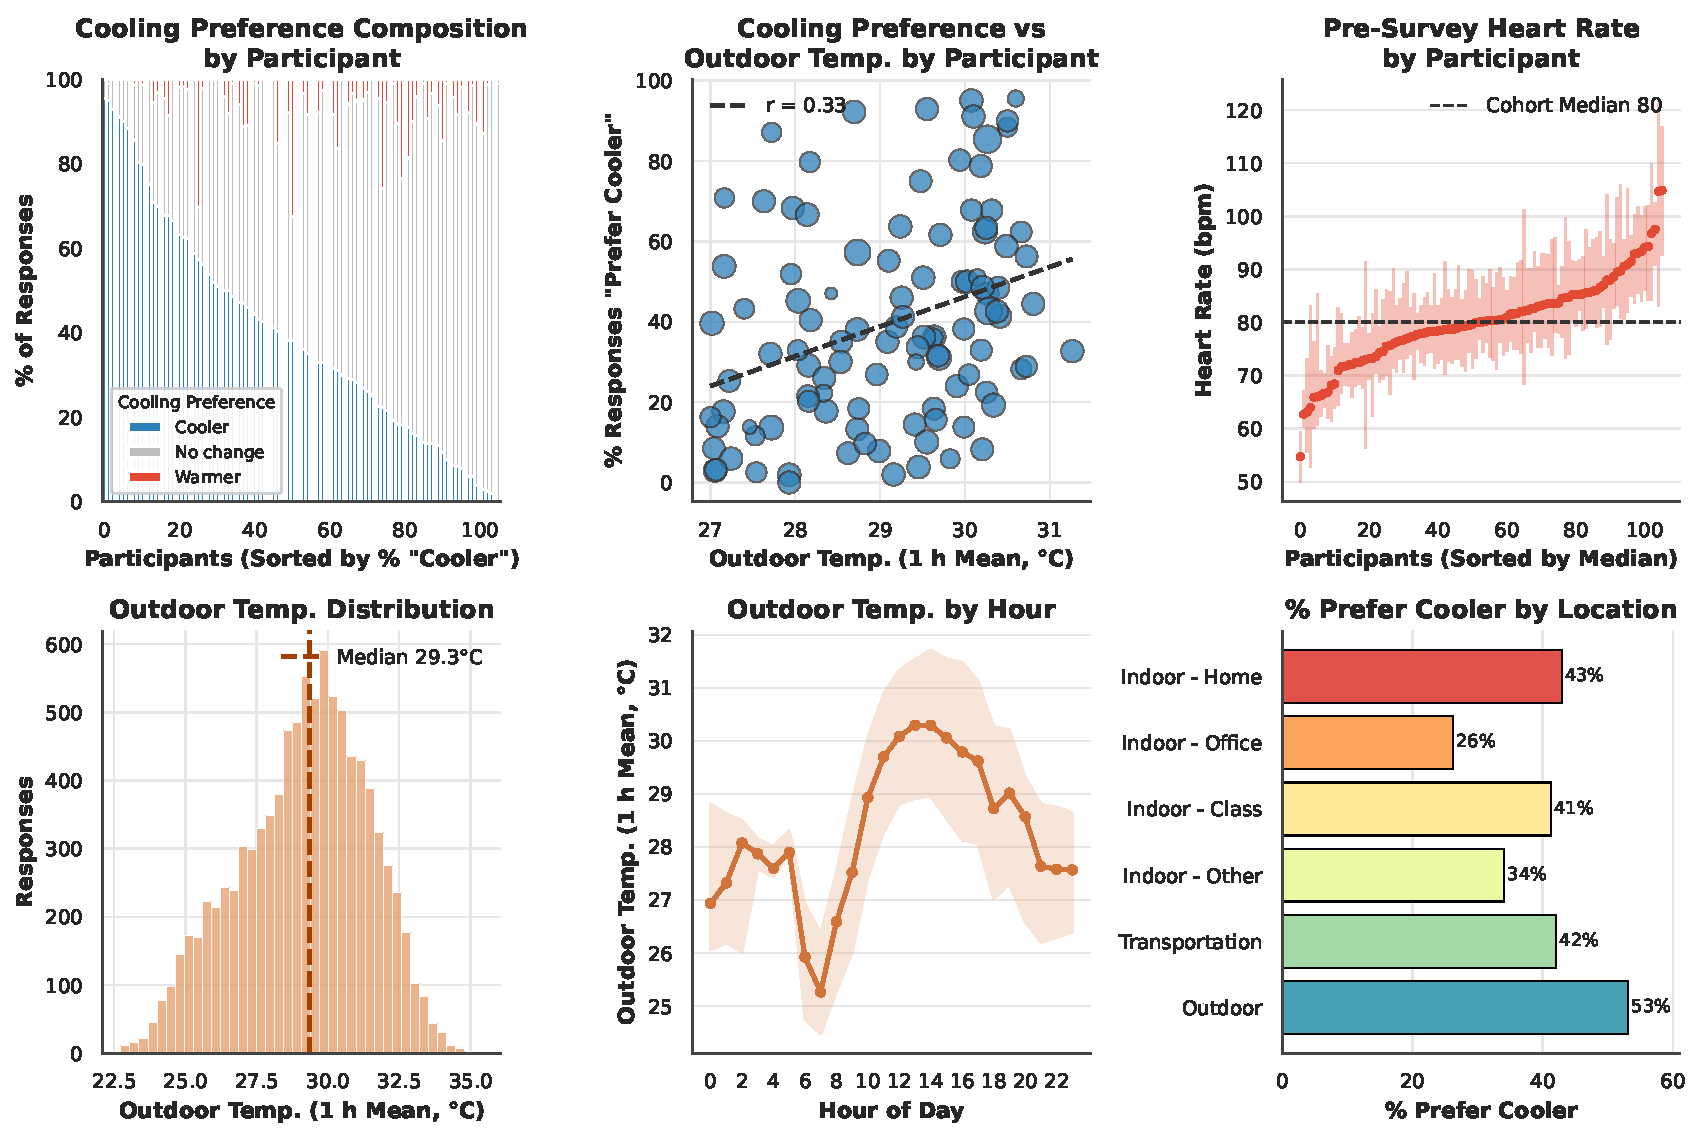
\includegraphics[width=\textwidth]{figures/data_characterization/cooling_preference.pdf}
% Detailed caption (archived): \caption{Participant-level and contextual patterns in cooling preference, arranged as a $2\times3$ grid. Top row: per-participant cooling-preference composition (stacked shares of cooler / no change / warmer, sorted by percent ``cooler''); the share preferring ``cooler'' against mean 1-hour pre-survey outdoor temperature by participant ($r = 0.33$); and per-participant pre-survey heart rate (cohort median 80\,bpm). Bottom row: the distribution of pre-survey outdoor temperature (median 29.3\,\textdegree C); outdoor temperature by hour of day; and the share preferring ``cooler'' by location type.}
\caption{Participant-level and contextual patterns in cooling preference, relating per-participant composition, outdoor temperature, heart rate, and location type.}
\label{fig:data-f2-cooling}
\end{figure}

% The source notebook identifies this visualization as Figure G1 (not G2).
\begin{figure}[htbp]
\centering
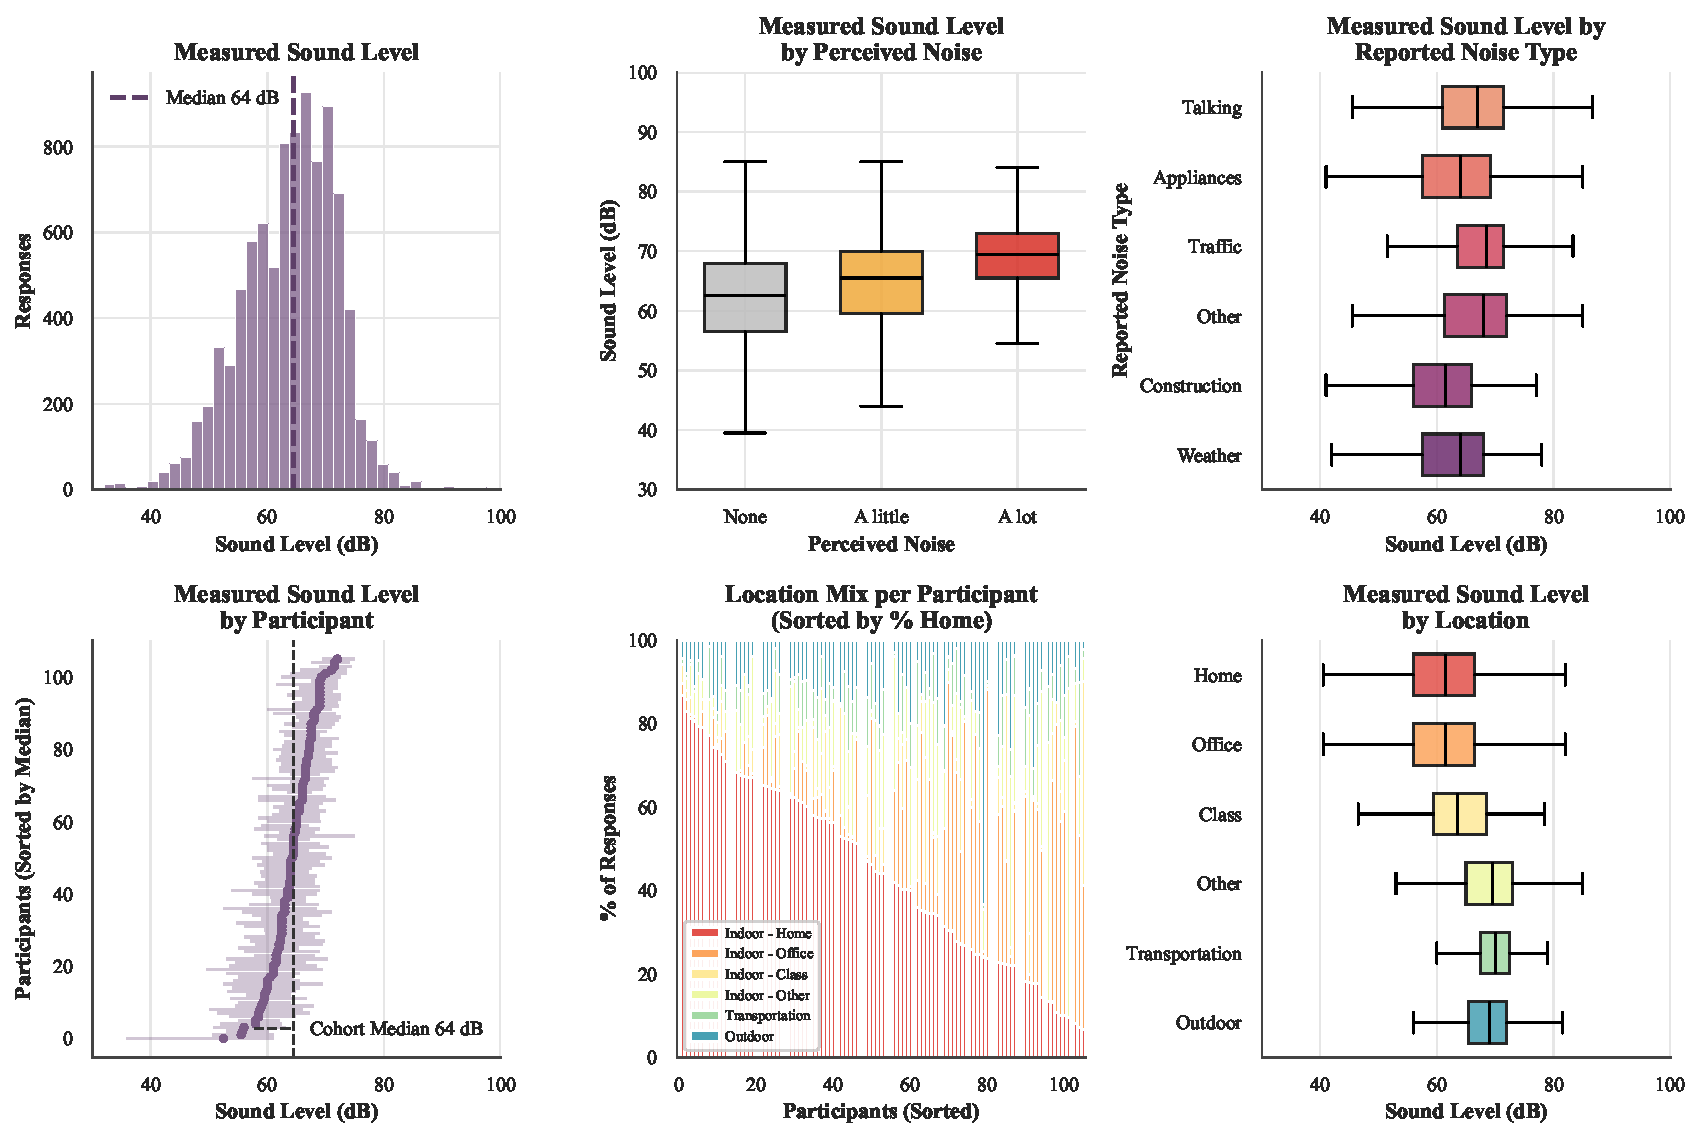
\includegraphics[width=\textwidth]{figures/data_characterization/noise_characterization.pdf}
% Detailed caption (archived): \caption{Measured sound level (1-hour pre-survey mean) across subjective, participant, and location contexts, arranged as a $2\times3$ grid. Top row: the overall distribution of measured sound level (median 64\,dB); measured sound level by perceived-noise answer (none / a little / a lot); and measured sound level by reported noise type. Bottom row: measured sound level by participant (sorted by median, cohort median 64\,dB); the location mix per participant (stacked space-type shares, sorted by percent home); and measured sound level by location type.}
\caption{Measured sound level (1-hour pre-survey mean) summarised across subjective, participant, and location contexts.}
\label{fig:data-g1-noise}
\end{figure}

\subsection{Perceptual fingerprints and association with space type}\label{sec:res-fingerprint-association}

With each perception characterized on its own, the analysis now asks how the reported experience differs across the spaces in which it was recorded.
It does so in three layers that build on one another.
The first layer, in Figure~\ref{fig:space-perception-fingerprint}, reads each space type as a profile by normalising within its own row.
Every cell gives the probability of a response given the space, so each row describes the mix of experiences in that setting rather than how many responses it contributed.
Read this way, the spaces separate into recognisable characters.
Home is a quiet, solitary setting, with most responses reporting \emph{None} for noise and about 84\% reporting \emph{Alone}, while classrooms and other-indoor spaces are mostly social.
The commute spaces stand out for discomfort, with the highest shares of \emph{A lot} of noise, reaching roughly one in four responses in transportation against only about 3\% at home.
Thermal preference shifts more gently, from only about a quarter of office responses wanting \emph{Cooler} to just over half of outdoor responses.
This fits the heavily air-conditioned office and the exposed outdoor setting, and it is a reminder that thermal preference reflects the immediate controlled environment more than the outdoor weather.
The fingerprint is intuitive but has one limit.
Because some responses are common everywhere, a high within-space probability does not by itself mean the response is characteristic of that space.

\begin{figure}[htbp]
\centering
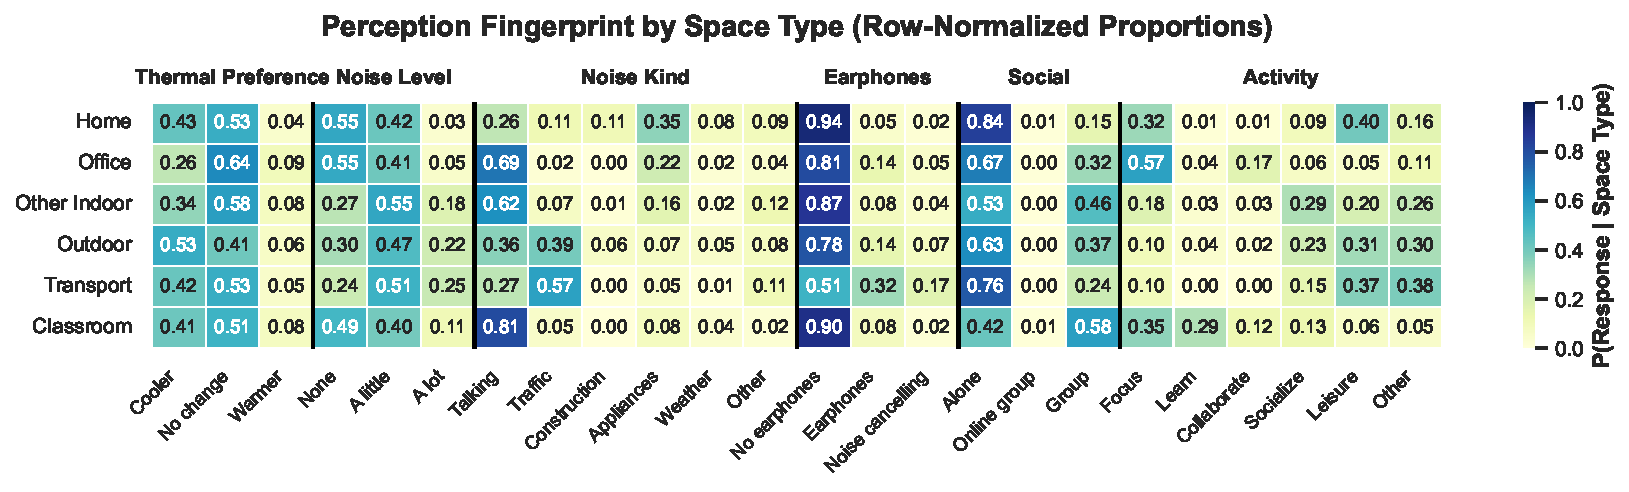
\includegraphics[width=\textwidth]{figures/data_characterization/perception_fingerprint_by_space_type.pdf}
% Detailed caption (archived): \caption{Conditional perception fingerprint by reported space type, drawn as a single heatmap. Rows are the six space types and columns are individual response options grouped by survey dimension (thermal preference, noise level, noise kind, earphones, social context, and activity). Each cell colour encodes $P(\mathrm{response}\mid\mathrm{space\ type})$, the within-space probability of that response, so that each row reads as the perceptual profile of one space type.}
\caption{Conditional perception fingerprint by space type in a heatmap of $P(\mathrm{response}\mid\mathrm{space\ type})$ with space types in rows and response options (grouped by survey dimension) in columns.}
\label{fig:space-perception-fingerprint}
\end{figure}

The second layer, in Figure~\ref{fig:space-perception-lift}, divides each within-space probability by the response's overall proportion in the dataset.
A lift above one marks a response that is more common in a space than in the data as a whole, and a lift below one marks one that is rarer.
This turns a profile into a signature, because it isolates what is distinctive to a space rather than what is simply frequent.
The contrast sharpens the same story and adds detail the fingerprint hides.
\emph{A lot} of noise is over-represented by about 2.6 times in transportation and 2.4 times outdoors, \emph{Group} is over-represented most in classrooms (lift near 2.1), and \emph{Warmer}, a rare response overall, is concentrated in the office (lift near 1.6) where air-conditioning can overshoot.
Lift also makes the source of noise a spatial fingerprint in its own right, as traffic accounts for most reported noise in transportation and a large share outdoors, while talking dominates the noise reported in classrooms and offices.
The limit of lift mirrors that of the fingerprint.
It flags distinctive combinations but does not show whether any single contrast is larger than chance would produce.

\begin{figure}[htbp]
\centering
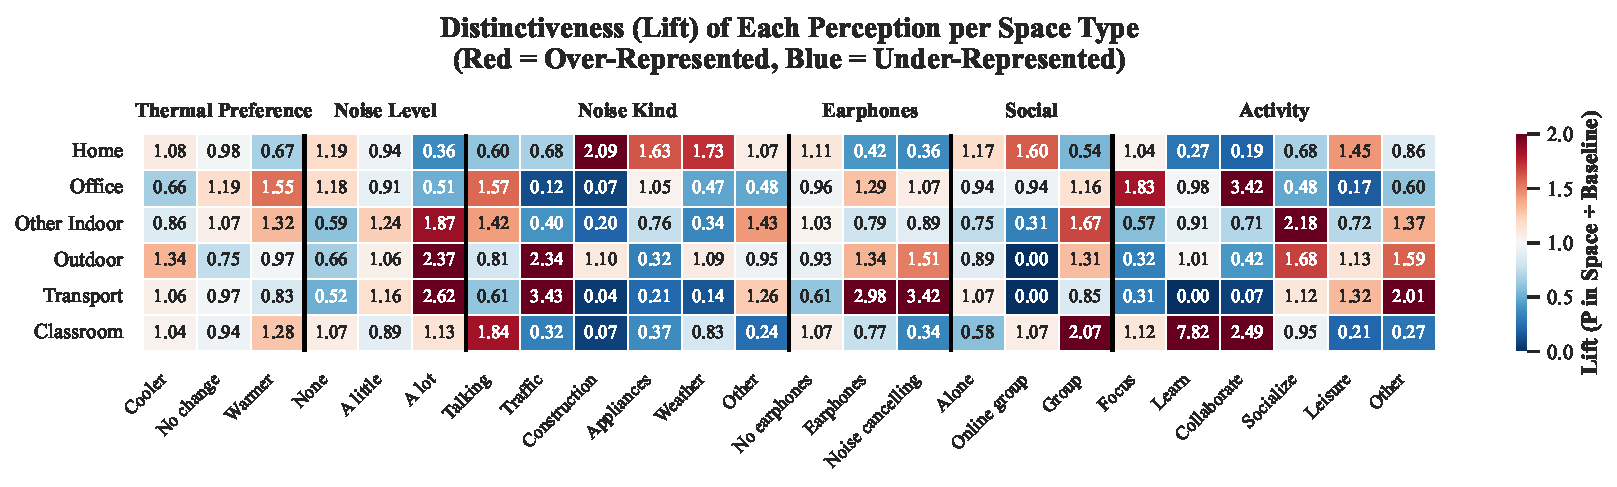
\includegraphics[width=\textwidth]{figures/data_characterization/perception_lift_by_space_type.pdf}
% Detailed caption (archived): \caption{Relative distinctiveness of perceptions by reported space type, drawn as a single heatmap with the same row (space type) and column (response option, grouped by dimension) layout as Figure~\ref{fig:space-perception-fingerprint}. Each cell shows lift, $P(\mathrm{response}\mid\mathrm{space\ type}) / P(\mathrm{response})$; values above one mark responses over-represented in a space relative to the whole dataset and values below one mark under-represented responses, isolating what is distinctive to a space rather than merely frequent.}
\caption{Relative distinctiveness of perceptions by space type, shown as lift, $P(\mathrm{response}\mid\mathrm{space\ type}) / P(\mathrm{response})$, with space types in rows and response options (grouped by survey dimension) in columns.}
\label{fig:space-perception-lift}
\end{figure}

Figure~\ref{fig:space-perception-residuals} illustrates the third layer of analysis that adds the statistical dimension the first two lack.
It compares each space and response combination against what independence would predict, using adjusted standardized residuals whose sign gives the direction of the effect and whose size is set on a standard-normal scale.
This layer confirms which distinctive contrasts are large relative to sampling noise, and it agrees with the overall effect sizes.
The association with space type is strongest for what a person is doing and hearing, with Cram\'er's V near $0.38$ for group activity, $0.35$ for solitary activity, and $0.28$ for the kind of noise, and weakest for thermal preference at about $0.12$.
The residuals make the behavioural picture explicit, as transportation and outdoor spaces stand out for loud, traffic-driven noise, classrooms and offices for talking and for group or focused activity, and home for quiet, solitary responses.
Thermal preference produces only muted residuals scattered across spaces.
Because the responses are clustered within 106 participants, the significance markers are read as descriptive screens rather than formal tests, and the agreement of all three layers on the same ordering is the stronger evidence.
The lesson across the three layers is that space type is written far more clearly into what people are doing and hearing than into how warm they feel.
This weak thermal signal is consistent with people often being in controlled indoor settings rather than exposed to the outdoor weather, and it is the central characterization result of the study.

\begin{figure}[htbp]
\centering
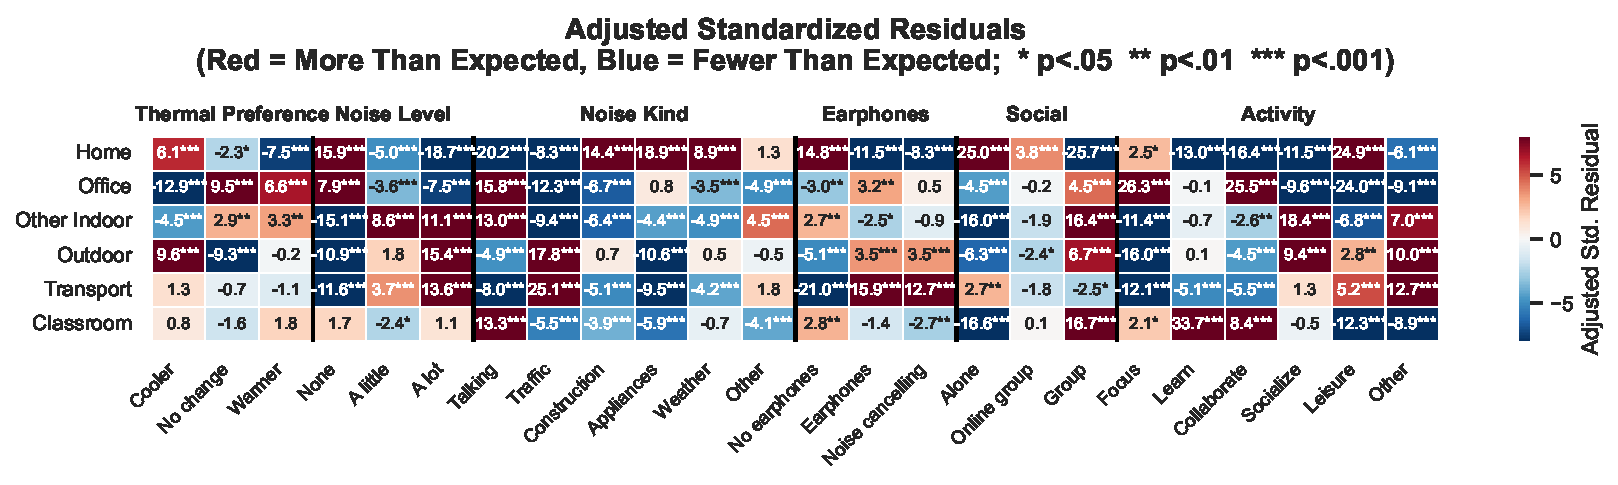
\includegraphics[width=\textwidth]{figures/data_characterization/perception_space_adjusted_residuals.pdf}
% Detailed caption (archived): \caption{Adjusted standardised residuals for space-type and perceptual-response combinations, drawn as a single heatmap sharing the row (space type) and column (response option, grouped by dimension) layout of Figures~\ref{fig:space-perception-fingerprint}--\ref{fig:space-perception-lift}. Cell colour gives each combination's departure from independence on a standard-normal scale: red cells occur more often than expected and blue cells less often, with larger magnitudes indicating stronger deviations.}
\caption{Adjusted standardised residuals for space-type by response combinations, where red cells occur more often and blue cells less often than expected under independence.}
\label{fig:space-perception-residuals}
\end{figure}

% \subsection{Multivariate, physiological, weather, and outdoor environmental patterns}\label{sec:res-multivariate-physio-outdoor}
% [PLACEHOLDER: Integrate the multivariate structure of subjective experience (MCA + k-modes) with physiological and weather signatures across space types. Then describe the outdoor-only environmental characterization, including streetscape and built-form profiles, their relationship with thermal preference, and the role of weather.]

% [PLACEHOLDER: Report the physiological gradient across spaces (sedentary Home to mobile Outdoor/Transport; steps largest effect), the weak ambient-weather signatures of space type, and the result that Outdoor is not necessarily the hottest reported space.]

% [PLACEHOLDER: Report the weather-versus-thermal-preference result: ``Cooler'' responses occur in genuinely hotter (higher heat-index) and drier conditions, while rain suppresses cooling demand. State the magnitude and limitations of this relationship.]


% \subsection{Discriminative modeling of space type}\label{sec:res-model}
% [PLACEHOLDER: Report the space-type classifier performance and feature importance
% (activity and noise-kind as strong space descriptors; ambient weather adds little).]


% ============================================================================
\section{Discussion}\label{sec:discussion}
% ============================================================================

The three analytical layers converge on a coherent characterization of how urban space types differ in reported experience.
The clearest separations are behavioural and acoustic rather than thermal: what people are doing and hearing identifies a space far more sharply than how warm they feel.
Tables~\ref{tab:insights-acoustic} and~\ref{tab:insights-social-thermal} collect the findings that reinforce prior expectation and establish this baseline character of each setting, grouped by the acoustic environment and by social context and thermal comfort.
Each entry pairs a short insight with the supporting detail drawn from the fingerprint, lift, and residual analyses of Section~\ref{sec:res-fingerprint-association}.

% Discussion 4.1 --- reinforcing findings: the acoustic environment.
\begin{table}[htbp]
\centering
\caption{Space-type findings that reinforce prior intuition: the acoustic environment.}
\label{tab:insights-acoustic}
\footnotesize
\renewcommand{\arraystretch}{1.3}
\begin{tabularx}{\textwidth}{@{}>{\raggedright\arraybackslash\bfseries}p{0.30\textwidth} >{\raggedright\arraybackslash}X@{}}
\toprule
\normalfont\textbf{Key insight} & \textbf{Detail} \\
\midrule
Commute spaces are the noisiest & Transportation and outdoor responses carry the highest \emph{a lot} noise shares ($\approx 25\%$ and $22\%$), against only about 3\% at home. \\
Home and offices are the quietest settings & Both sit near a 62\,dB median sound level, the lowest among the measured spaces. \\
Perceived loudness tracks the setting & Louder spaces attract more \emph{a lot} noise reports, so subjective loudness follows the physical environment. \\
Traffic defines commute noise & Traffic is the dominant reported noise source in transportation ($\approx 57\%$) and outdoors ($\approx 39\%$). \\
Talking defines indoor noise & Talking dominates the acoustic complaints of classrooms ($\approx 81\%$) and offices ($\approx 69\%$). \\
\bottomrule
\end{tabularx}
\end{table}

% Discussion 4.1 --- reinforcing findings: social context and thermal comfort.
\begin{table}[htbp]
\centering
\caption{Space-type findings that reinforce prior intuition: social context and thermal comfort. Details are drawn from the fingerprint, lift, and residual analyses of Section~\ref{sec:res-fingerprint-association}.}
\label{tab:insights-social-thermal}
\footnotesize
\renewcommand{\arraystretch}{1.3}
\begin{tabularx}{\textwidth}{@{}>{\raggedright\arraybackslash\bfseries}p{0.30\textwidth} >{\raggedright\arraybackslash}X@{}}
\toprule
\normalfont\textbf{Key insight} & \textbf{Detail} \\
\midrule
Home is overwhelmingly solitary & About 84\% of home responses report being \emph{alone}, the most solitary setting measured. \\
Classrooms are the most social setting & Classrooms are the most group-oriented space, with a group lift near 2.1. \\
Activity is the strongest spatial marker & Group activity is the response most tightly associated with space type (Cram\'er's V $\approx 0.38$). \\
Offices show the lowest cooling demand & Only about 26\% of office responses want \emph{cooler}, consistent with heavy air-conditioning. \\
Outdoor spaces show the highest cooling demand & Just over half ($\approx 53\%$) of outdoor responses want \emph{cooler}. \\
\bottomrule
\end{tabularx}
\end{table}


These reinforcing findings matter less as surprises than as evidence that a watch-based micro-survey recovers the settled structure of urban experience that the field has documented through other instruments.
Urban research has increasingly treated residents' perceptions of their surroundings as a primary measurement in their own right rather than as a noisy proxy for physical conditions, on the argument that how people read an environment can matter more for outcomes such as self-rated health than the measured environment itself \citep{Kim2016-wx}.
Capturing those perceptions at the scale of a city has motivated a parallel line of mobile-crowdsourcing work, in which residents contribute geolocated subjective reports---of safety, comfort, or nuisance---from their own devices as they move through the urban fabric \citep{Phuttharak2020-js}.
The present study sits within this tradition and extends it by delivering the survey on the wrist and pairing each response with onboard sensing, so that the solitary-quiet character of home and the social character of classrooms emerge from in-situ reports rather than from recalled or remotely elicited judgements.

The acoustic results align closely with what this body of work has found through other means.
That commute spaces carry the highest \emph{a lot} noise shares and that traffic dominates their reported noise source echoes mobile-exposure studies of commuters, in which personal exposure to traffic-driven noise and air pollution is highly context-dependent and is best captured by combining wearable measurement with in-situ, on-the-move accounts \citep{Marquart2022-rt}.
It is equally consistent with spatio-temporal urban assessments that locate the loudest ambient conditions in traffic-dense cores rather than in the residential or green periphery \citep{Kumar2013-if}.
The convergence of a wrist-based micro-survey with dosimetry-, interview-, and remote-sensing-based approaches on the same ordering of spaces is more informative than any single instrument would be, and it is the kind of cross-method corroboration that motivates treating the quieter findings that follow as trustworthy.

Methodologically, the layered reading of subjective, physiological, and spatial signals used here belongs to a growing strand of multi-method urban perception research, exemplified by integrations of participatory mapping, neurophysiological response, and self-reported emotion to characterise experiences such as perceived walkability \citep{Yildirim2026-rg}.
Within the specific pairing of thermal and acoustic experience, the watch-based platform used here has already supported city-scale prediction of noise distraction and thermal preference \citep{Miller2025-qu}, and the characterization below establishes the descriptive structure on which such predictive work rests.

Beyond this expected picture, several results are less obvious and reshape how the characterization should be read.
Thermal preference, the signal one might expect a tropical climate to dominate, is in fact the weakest spatial marker, while distinctiveness that raw proportions understate emerges only once responses are weighed against their overall frequency.
Tables~\ref{tab:insights-counterintuitive} and~\ref{tab:insights-behaviour} gather these counterintuitive and analytical findings, separating the environmental and thermal surprises from the behavioural signatures and from the framing that effect sizes, rather than p-values, provide under participant nesting.

% Discussion 4.2 --- counterintuitive environmental and thermal signals.
\begin{table}[htbp]
\centering
\caption{Counterintuitive environmental and thermal signals.}
\label{tab:insights-counterintuitive}
\footnotesize
\renewcommand{\arraystretch}{1.3}
\begin{tabularx}{\textwidth}{@{}>{\raggedright\arraybackslash\bfseries}p{0.30\textwidth} >{\raggedright\arraybackslash}X@{}}
\toprule
\normalfont\textbf{Key insight} & \textbf{Detail} \\
\midrule
Thermal preference is the weakest spatial signal & Its association with space type (Cram\'er's V $\approx 0.12$) sits far below activity or noise. \\
Cooling demand separates spaces only modestly & Outdoor demand ($\approx 53\%$) exceeds home ($\approx 43\%$) by less than an air-conditioning-driven intuition would suggest. \\
Offices can over-cool & Wanting \emph{warmer}, rare overall, concentrates in offices (lift $\approx 1.6$), a signature of air-conditioning overshoot. \\
The kind of noise matters more than the amount & The source of noise fingerprints a space more sharply than how loud it is. \\
Lift exposes hidden distinctiveness & \emph{A lot} of noise is $\approx 2.6\times$ over-represented in transportation relative to the whole corpus, a contrast raw proportions understate. \\
\bottomrule
\end{tabularx}
\end{table}

% Discussion 4.2 --- behavioral signatures and analytical framing.
\begin{table}[htbp]
\centering
\caption{Behavioral signatures and analytical framing.}
\label{tab:insights-behaviour}
\footnotesize
\renewcommand{\arraystretch}{1.3}
\begin{tabularx}{\textwidth}{@{}>{\raggedright\arraybackslash\bfseries}p{0.30\textwidth} >{\raggedright\arraybackslash}X@{}}
\toprule
\normalfont\textbf{Key insight} & \textbf{Detail} \\
\midrule
Behavior separates spaces best & What a person is doing distinguishes space types more sharply than any environmental variable. \\
Home is distinctively, not just frequently, solitary & Even against an already alone-dominated corpus, home's alone lift exceeds one. \\
Commuting is loud and lonely & Transportation pairs loud, traffic-driven noise with high solitude ($\approx 76\%$ alone), combining discomfort with isolation. \\
Three methods converge & Fingerprint, lift, and residuals agree on the same behavioral ordering, strengthening confidence beyond any single test. \\
Effect sizes, not p-values, are the valid read-out & Responses are nested within 106 participants, so significance markers act as descriptive screens rather than formal tests. \\
\bottomrule
\end{tabularx}
\end{table}


\subsection{Implications for sustainable urban design}\label{sec:disc-implications}
% [PLACEHOLDER: Connect findings to the journal scope --- what they mean for
% thermal-comfort-aware, health-supportive and energy-conscious urban design and
% policy in tropical cities.]
The results of this analysis support the ability to close the loop between the design of how planners predict occupants behave and perceive their environment versus how they actually do in the real world. 
Much of the insights reinforce intuition, but there could be subregions that perform better or worse than expected.
Heat and noise are two elements that are characterized, but numerous other subjective elements can be captured.

\subsection{Limitations}\label{sec:disc-limitations}
% [PLACEHOLDER: Participant nesting / pseudoreplication; ambient nearest-station
% weather as a coarse proxy for personal exposure; convenience sample; Singapore-
% specific A/C context; self-reported perceptions.]
Sample size and lack of diversity of participants make it difficult for these insights to be generalized across the population.
Convenience sampling and lack or sensors.

\subsection{Future work}\label{sec:disc-future}
% [PLACEHOLDER: Directions --- personal microclimate sensing, larger/more diverse
% cohorts, cross-city replication, mixed-effects modeling accounting for
% participant nesting.]
Deeper characterization of the subset of the population that have certain parterns of behavior would help estabblish archetypes of behavior to identify which should be reinforced versus prevented from becoming ubiquitous. 
Targeted microsurveys based on where the person is and waht the subjective target of the deployment is.
Development of larger deployments across people who have thier own smartwatch to result in possibly thousands or more participants.



% ============================================================================
\section{Conclusion}\label{sec:conclusion}
% ============================================================================
[PLACEHOLDER: Concise restatement of the contribution and headline takeaway for
sustainable urban development.]


% ============================================================================
\section*{Acknowledgements}
% ============================================================================
The authors acknowledge the student researchers who assisted with data collection and processing: Charis Boey, Kristi Maisha, Annabel Sim, Aisyah Iskandar, Lum Jun Chao, and S Aravindkugesh.

\section*{CRediT authorship contribution statement}
Clayton Miller: Visualization, Software, Resources, Methodology, Funding acquisition, Formal analysis, Writing -- original draft, Supervision, Project administration, Investigation, Conceptualization. Mario Frei: Writing -- review \& editing, Validation, Project administration, Investigation, Conceptualization, Methodology, Data curation. Yun Xuan Chua: Methodology, Conceptualization, Writing -- review \& editing, Project administration, Investigation. 

\section*{Declaration of generative AI use}
The authors used Runcell AI, powered by OpenAI's GPT-5.6 Terra large language model, and Claude Opus 4.8 by Anthropic to assist with the organisation of the \LaTeX{} manuscript, figure placement, and language polishing. These tools were not used to generate the study data, conduct the analysis, or replace the authors' scholarly judgement. All generated suggestions were reviewed and revised by the authors, who take full responsibility for the originality, accuracy, integrity, citations, and final content of this manuscript. Generative AI is not listed as an author.

\section*{Disclosure statement}
The authors declare that they have no known competing financial interests or personal relationships that could have appeared to influence the work reported in this paper.

\section*{Funding}
This research was supported by the Singapore Ministry of Education (MOE) Tier 1 Grants titled \textit{The Internet-of-Buildings (IoB) Platform -- Testing of Visual Analytics for AI Technologies towards a Well and Green Built Environment} (A-0008305-01-00) and Ecological Momentary Assessment (EMA) for Built Environment Research (A0008301-01-00).

\section*{Data availability statement}
The data and code supporting the findings of this study will be available on GitHub. 
% [PLACEHOLDER: Insert the permanent repository URL and DOI, if available.]


% ============================================================================
% References
% ============================================================================
% Citation keys are maintained in cozie_singapore_references.bib. For example:
% \citep{Tartarini2023-iu,Kirchner2016-dq,Kingsbury2024-qe}
\bibliographystyle{apacite}% Taylor & Francis APA-style (matches the interact sample)
\bibliography{cozie_sg}

\end{document}
